\section{\textbf{APPENDIX CIRCLE CURVE}} \label{APPENDIX CIRCLE CURVE}

\subsection       {Plot of Circle curve
[\ref      {01-img-Plot of Circle curve.pdf} ] }
\label{ssec-01-img-Plot of Circle curve.pdf}

\subsection       {Circle Radius of Curvature
[\ref      {02-img-Circle Radius of Curvature.pdf}] }
\label{ssec-02-img-Circle Radius of Curvature.pdf}

\subsection       {Circle Validation in LinuxCNC
[\ref      {03-img-Circle-Validation-in-LinuxCNC.png} ] }
\label{ssec-03-img-Circle-Validation-in-LinuxCNC.png}

\subsection     {Circle Direction of Travel 3D
[\ref      {04-img-Circle Direction of Travel 3D.pdf} ] }
\label{ssec-04-img-Circle Direction of Travel 3D.pdf}

\subsection       {Circle First and Second Order Taylor's Approx
[\ref      {05-img-Circle-First-and-Second-Order-Taylors-Approx.pdf}] }
\label{ssec-05-img-Circle-First-and-Second-Order-Taylors-Approx.pdf}

\subsection       {Circle First minus Second Order Taylor's Approx
[\ref      {06-img-Circle-First-minus-Second-Order-Taylors-Approx.pdf}] }
\label{ssec-06-img-Circle-First-minus-Second-Order-Taylors-Approx.pdf}

\subsection       {Circle Separate First and Second Order Taylor's Approx
[\ref      {07-img-Circle-Separation-First-and-Second-Order-Taylors-Approx.pdf} ] }
\label{ssec-07-img-Circle-Separation-First-and-Second-Order-Taylors-Approx.pdf}

\subsection       {Circle Separation SAL and SCL
[\ref      {08-img-Circle-Separation-SAL-and-SCL.pdf}] }
\label{ssec-08-img-Circle-Separation-SAL-and-SCL.pdf}

\subsection       {Circle Chord-error in close view 2 scales
[\ref      {09-img-Circle-Chord-error-in-close-view-2-scales.pdf}] }
\label{ssec-09-img-Circle-Chord-error-in-close-view-2-scales.pdf}

\subsection       {Circle Four Components Feedrate Limit
[\ref      {10-img-Circle-Four-Components-Feedrate-Limit.pdf} ] }
\label{ssec-10-img-Circle-Four-Components-Feedrate-Limit.pdf}

\subsection    {Circle FrateCommand FrateLimit and Curr-Frate
[\ref      {11-img-Circle-FrateCommand-FrateLimit-and-Curr-Frate.pdf}] }
\label{ssec-11-img-Circle-FrateCommand-FrateLimit-and-Curr-Frate.pdf}

\subsection     {Circle FeedRateLimit minus CurrFeedRate
[\ref      {12-img-Circle-FeedRateLimit-minus-CurrFeedRate.pdf} ] }
\label{ssec-12-img-Circle-FeedRateLimit-minus-CurrFeedRate.pdf}

\subsection     {Circle FC20-Nominal X and Y Feedrate Profiles
[\ref      {13-img-Circle-FC20-Nominal-X-and-Y-Feedrate-Profiles.pdf} ] }
\label{ssec-13-img-Circle-FC20-Nominal-X-and-Y-Feedrate-Profiles.pdf}

\subsection     {Circle FC20 Nominal Tangential Acceleration
[\ref      {14-img-Circle-FC20-Nominal-Tangential-Acceleration.pdf} ] }
\label{ssec-14-img-Circle-FC20-Nominal-Tangential-Acceleration.pdf}

\subsection     {Circle FC20 Nominal Rising S-Curve Profile
[\ref      {15-img-Circle-FC20-Nominal-Rising-S-Curve-Profile.pdf} ] }
\label{ssec-15-img-Circle-FC20-Nominal-Rising-S-Curve-Profile.pdf}

\subsection     {Circle FC20 Nominal Falling S-Curve Profile
[\ref      {16-img-Circle-FC20-Nominal-Falling-S-Curve-Profile.pdf}] }
\label{ssec-16-img-Circle-FC20-Nominal-Falling-S-Curve-Profile.pdf}

\subsection       {Circle FC10 Colored Feedrate Profile data ngcode
[\ref      {17-img-Circle-FC10-Colored-Feedrate-Profile-data_ngcode.png} ] }
\label{ssec-17-img-Circle-FC10-Colored-Feedrate-Profile-data_ngcode.png}

\subsection       {Circle FC20 Colored Feedrate Profile data ngcode
[\ref      {18-img-Circle-FC20-Colored-Feedrate-Profile-data_ngcode.png} ] }
\label{ssec-18-img-Circle-FC20-Colored-Feedrate-Profile-data_ngcode.png}

Continue ...\\

\subsection       {Circle FC30 Colored Feedrate Profile data ngcode
[\ref      {19-img-Circle-FC30-Colored-Feedrate-Profile-data_ngcode.png} ] }
\label{ssec-19-img-Circle-FC30-Colored-Feedrate-Profile-data_ngcode.png}

\subsection       {Circle FC40 Colored Feedrate Profile data ngcode
[\ref      {20-img-Circle-FC40-Colored-Feedrate-Profile-data_ngcode.png} ] }
\label{ssec-20-img-Circle-FC40-Colored-Feedrate-Profile-data_ngcode.png}

\subsection       {Circle FC10 Tangential Acceleration
[\ref      {21-img-Circle-FC10-Tangential-Acceleration.pdf}] }
\label{ssec-21-img-Circle-FC10-Tangential-Acceleration.pdf}

\subsection       {Circle FC20 Tangential Acceleration
[\ref      {22-img-Circle-FC20-Tangential-Acceleration.pdf}] }
\label{ssec-22-img-Circle-FC20-Tangential-Acceleration.pdf}

\subsection       {Circle FC30 Tangential Acceleration
[\ref      {23-img-Circle-FC30-Tangential-Acceleration.pdf}] }
\label{ssec-23-img-Circle-FC30-Tangential-Acceleration.pdf}

\subsection       {Circle FC40 Tangential Acceleration
[\ref      {24-img-Circle-FC40-Tangential-Acceleration.pdf}] }
\label{ssec-24-img-Circle-FC40-Tangential-Acceleration.pdf}

\subsection       {Circle FC20 Nominal Separation NAL and NCL
[\ref      {25-img-Circle-FC20-Nominal-Separation-NAL-and-NCL.pdf}] }
\label{ssec-25-img-Circle-FC20-Nominal-Separation-NAL-and-NCL.pdf}

\subsection       {Circle SAL minus SCL for FC10 FC20 FC30 FC40
[\ref      {26-img-Circle-Difference-SAL-minus-SCL-for-FC10-FC20-FC30-FC40.pdf}] }
\label{ssec-26-img-Circle-Difference-SAL-minus-SCL-for-FC10-FC20-FC30-FC40.pdf}


\subsection       {Circle FC10 FrateCmd CurrFrate X-Frate Y-Frate
[\ref      {27-img-Circle-FC10-FrateCmd-CurrFrate-X-Frate-Y-Frate.pdf}] }
\label{ssec-27-img-Circle-FC10-FrateCmd-CurrFrate-X-Frate-Y-Frate.pdf}

\subsection       {Circle FC20 FrateCmd CurrFrate X-Frate Y-Frate
[\ref      {28-img-Circle-FC20-FrateCmd-CurrFrate-X-Frate-Y-Frate.pdf}] }
\label{ssec-28-img-Circle-FC20-FrateCmd-CurrFrate-X-Frate-Y-Frate.pdf}

\subsection       {Circle FC30 FrateCmd CurrFrate X-Frate Y-Frate
[\ref      {29-img-Circle-FC30-FrateCmd-CurrFrate-X-Frate-Y-Frate.pdf}] }
\label{ssec-29-img-Circle-FC30-FrateCmd-CurrFrate-X-Frate-Y-Frate.pdf}

\subsection       {Circle FC40 FrateCmd CurrFrate X-Frate Y-Frate
[\ref      {30-img-Circle-FC40-FrateCmd-CurrFrate-X-Frate-Y-Frate.pdf}] }
\label{ssec-30-img-Circle-FC40-FrateCmd-CurrFrate-X-Frate-Y-Frate.pdf}

\subsection       {Circle FC10 Four Components FeedrateLimit
[\ref      {31-img-Circle-FC10-Four-Components-FeedrateLimit.pdf}] }
\label{ssec-31-img-Circle-FC10-Four-Components-FeedrateLimit.pdf}

\subsection       {Circle FC20 Four Components FeedrateLimit
[\ref      {32-img-Circle-FC20-Four-Components-FeedrateLimit.pdf}] }
\label{ssec-32-img-Circle-FC20-Four-Components-FeedrateLimit.pdf}

\subsection       {Circle FC30 Four Components FeedrateLimit
[\ref      {33-img-Circle-FC30-Four-Components-FeedrateLimit.pdf}] }
\label{ssec-33-img-Circle-FC30-Four-Components-FeedrateLimit.pdf}

\subsection       {Circle FC40 Four Components FeedrateLimit
[\ref      {34-img-Circle-FC40-Four-Components-FeedrateLimit.pdf}]}
\label{ssec-34-img-Circle-FC40-Four-Components-FeedrateLimit.pdf}

\subsection       {Circle Histogram Points FC10 FC20 FC30 FC40
[\ref       {35-img-Circle-Histogram-Points-FC10-FC20-FC30-FC40.pdf}] }
\label{ssec-35-img-Circle-Histogram-Points-FC10-FC20-FC30-FC40.pdf}

\subsection    {Circle Table distribution of interpolated points
[\ref      {tab-Circle Table distribution of interpolated points}] }
\label{ssec-tab-Circle Table distribution of interpolated points}

\subsection          {Circle Table FC10-20-30-40 Run Performance data
[\ref       {tab-app4-Circle-Table-FC10-20-30-40-Run-Performance-data} ] }
\label{ssec-tab-app4-Circle-Table-FC10-20-30-40-Run-Performance-data}


%% =====================================================
%% ==================================================
\clearpage
\pagebreak

\begin{figure}
	\caption     {Plot of Circle curve}
	\label{01-img-Plot of Circle curve.pdf}
	%%	\centering
	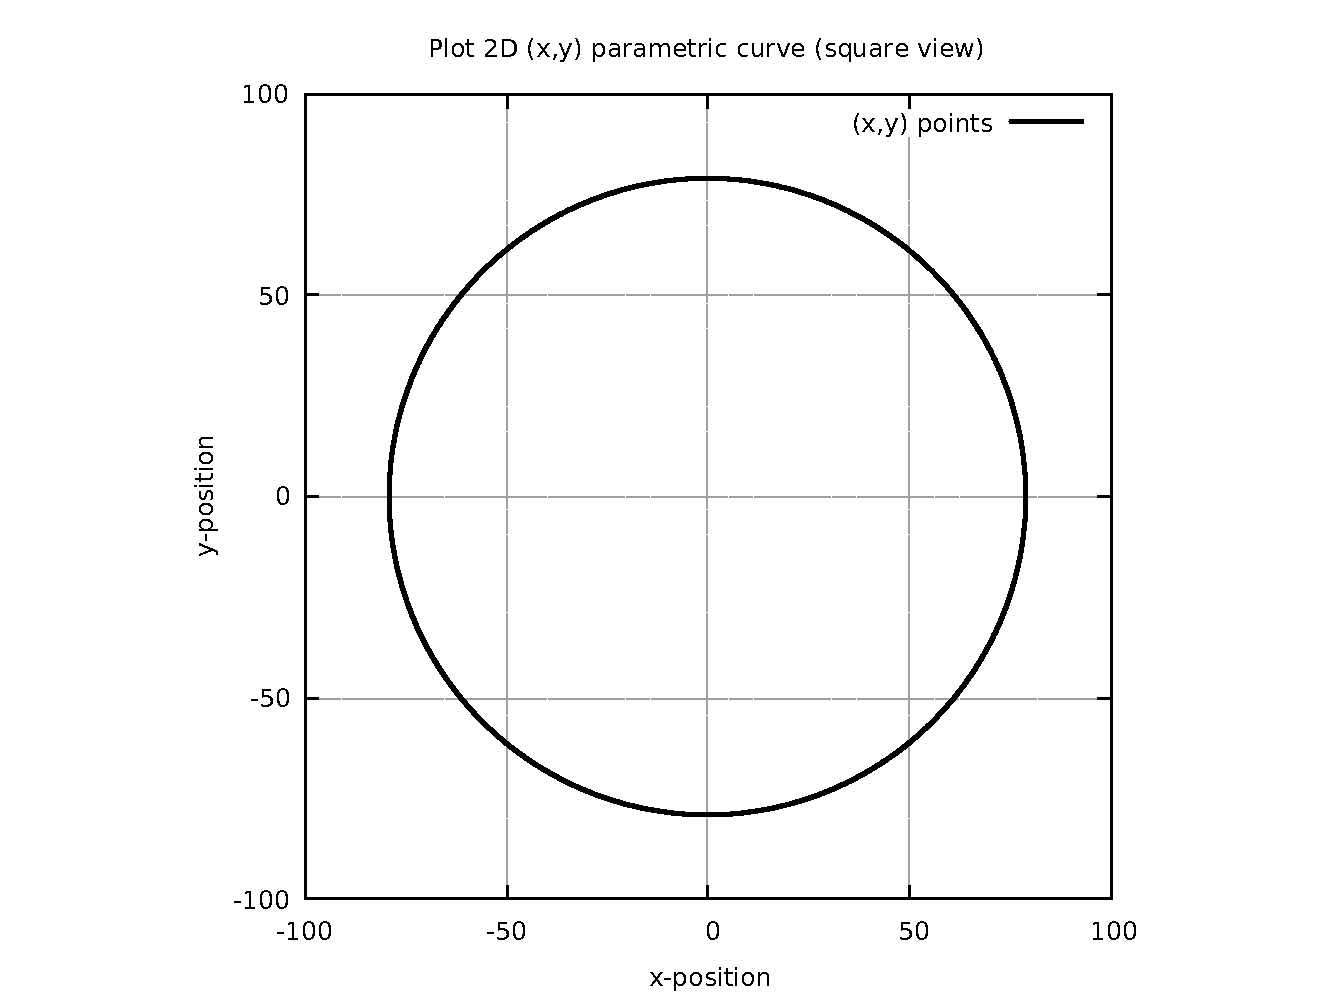
\includegraphics[width=1.00\textwidth]{Chap4/appendix/app-Circle/plots/01-img-Plot of Circle curve.pdf}
\end{figure}	


\begin{figure}
	\caption     {Circle Radius of Curvature}
	\label{02-img-Circle Radius of Curvature.pdf}
	%%	\centering
	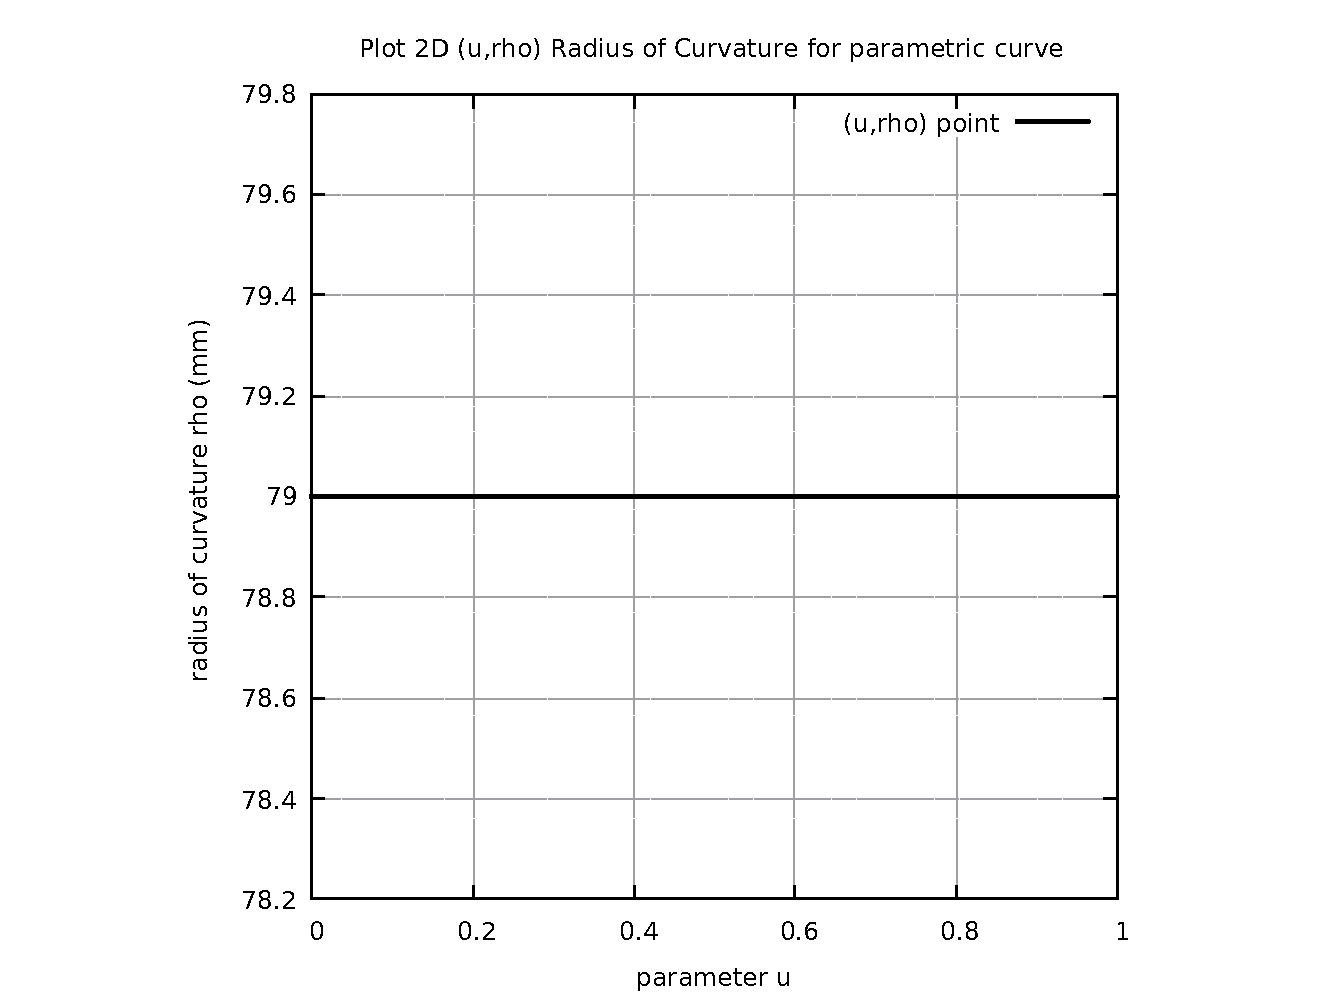
\includegraphics[width=1.00\textwidth]{Chap4/appendix/app-Circle/plots/02-img-Circle Radius of Curvature.pdf} 
\end{figure}	


%% ==================================================
\clearpage
\pagebreak

\begin{figure}
	\caption     {Circle Validation in LinuxCNC}
	\label{03-img-Circle-Validation-in-LinuxCNC.png}
	%%	\centering
	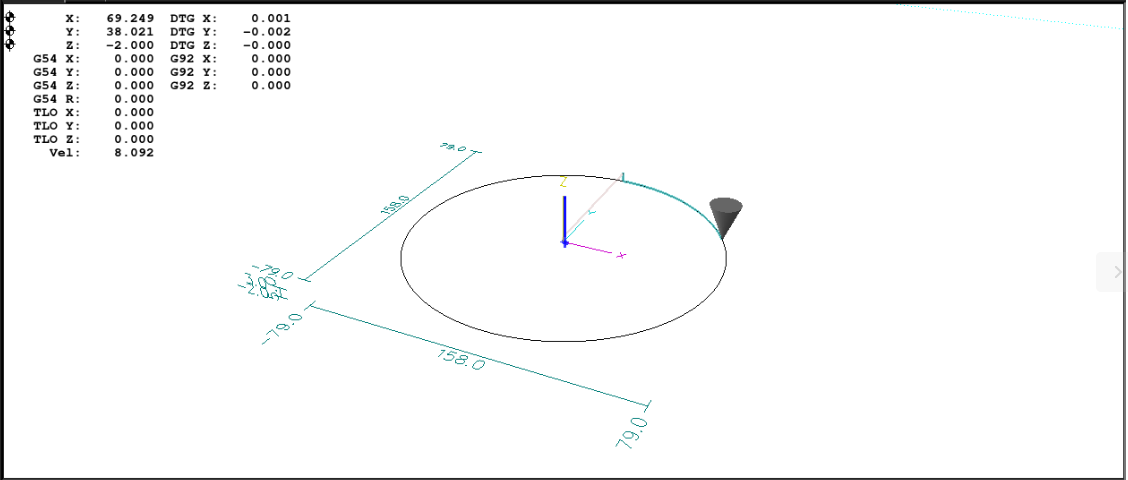
\includegraphics[width=1.00\textwidth]{Chap4/appendix/app-Circle/plots/03-img-Circle-Validation-in-LinuxCNC.png}
\end{figure}


\begin{figure}
	\caption     {Circle Direction of Travel 3D}
	\label{04-img-Circle Direction of Travel 3D.pdf}
	%%	\centering
	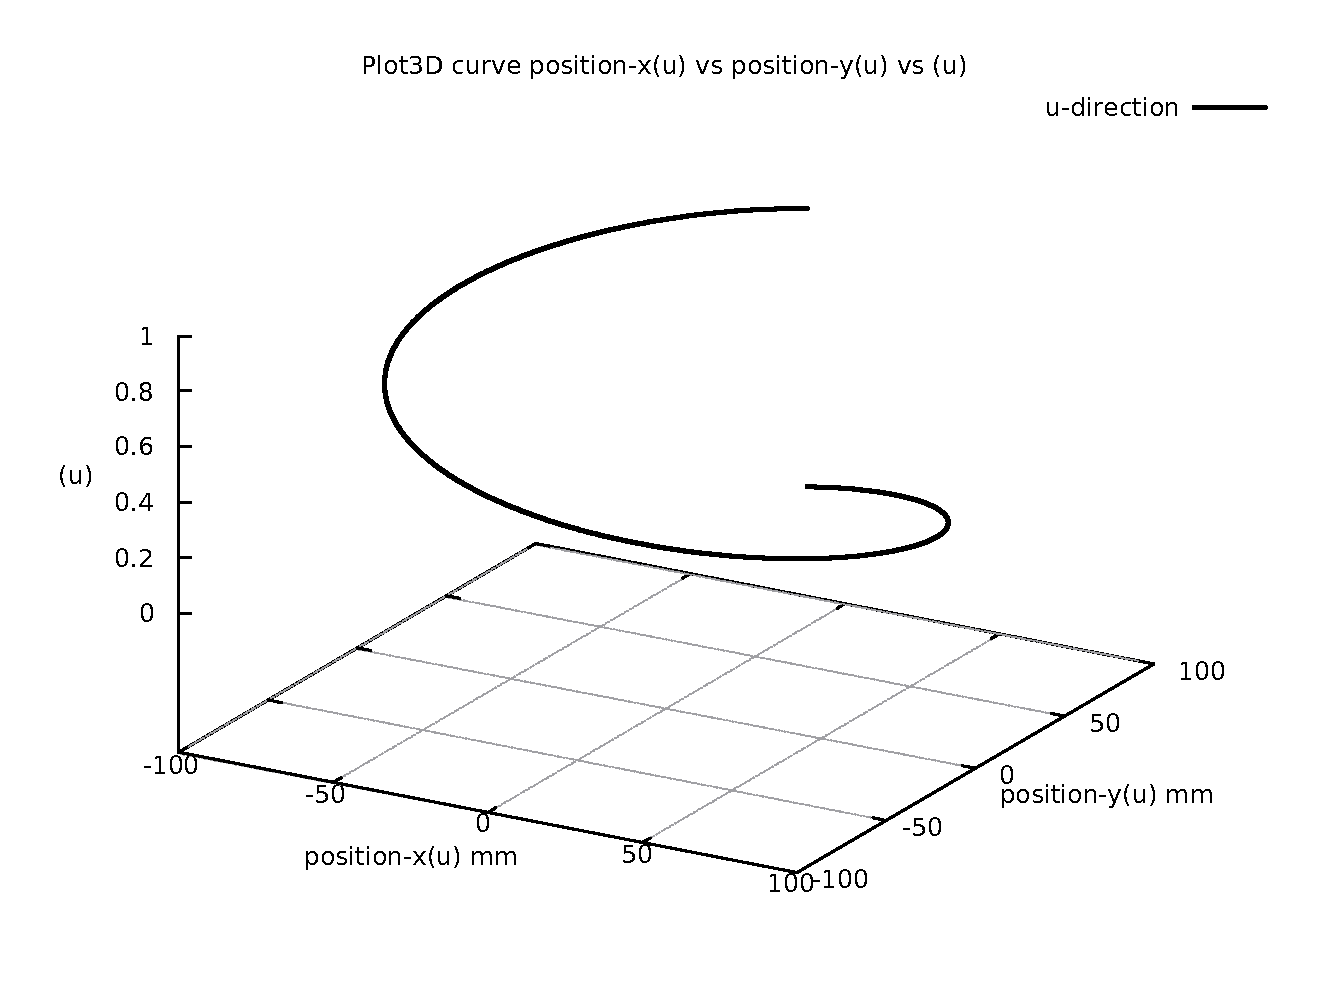
\includegraphics[width=1.00\textwidth]{Chap4/appendix/app-Circle/plots/04-img-Circle Direction of Travel 3D.pdf}
\end{figure}

%% ==================================================
\clearpage
\pagebreak

\begin{figure}
	\caption     {Circle First and Second Order Taylor's Approximation}
	\label{05-img-Circle-First-and-Second-Order-Taylors-Approx.pdf}
	%%	\centering
	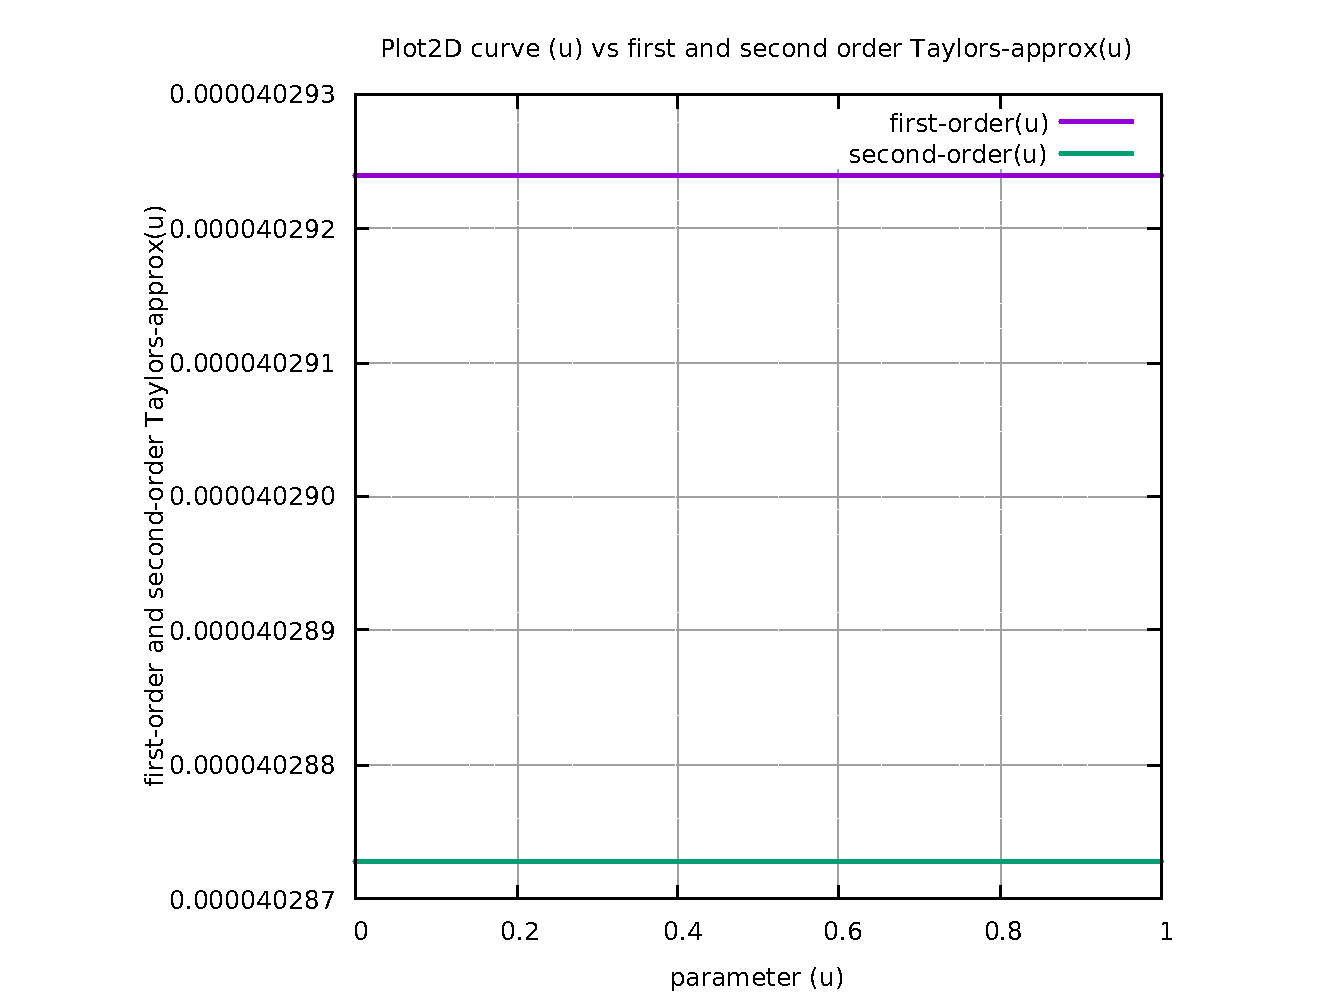
\includegraphics[width=1.00\textwidth]{Chap4/appendix/app-Circle/plots/05-img-Circle-First-and-Second-Order-Taylors-Approx.pdf}
\end{figure}


\begin{figure}
	\caption     {Circle First minus Second Order Taylor's Approximation}
	\label{06-img-Circle-First-minus-Second-Order-Taylors-Approx.pdf}
	%%	\centering
	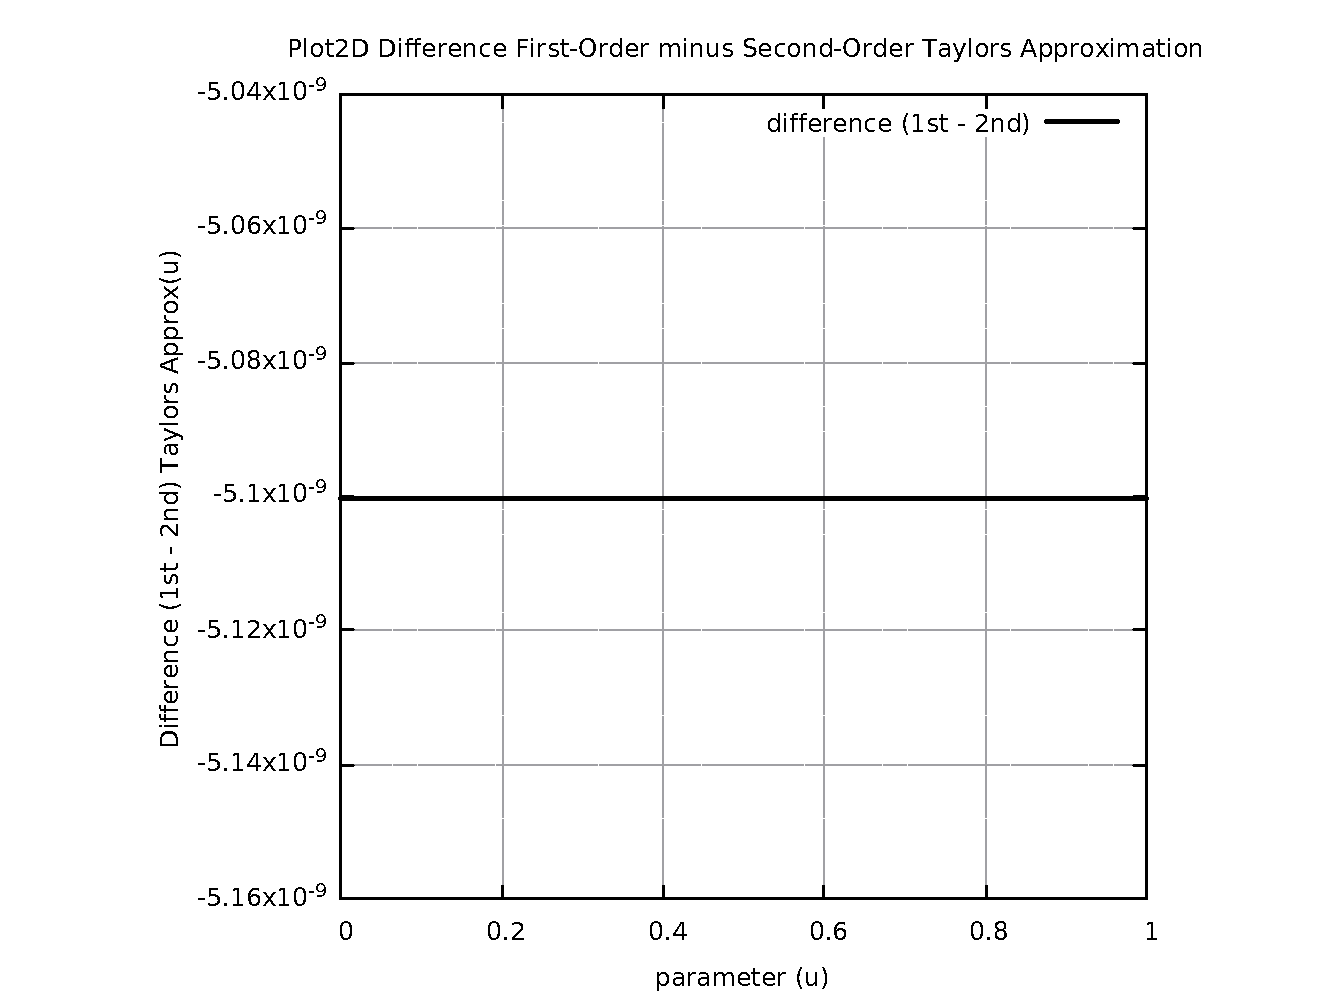
\includegraphics[width=1.00\textwidth]{Chap4/appendix/app-Circle/plots/06-img-Circle-First-minus-Second-Order-Taylors-Approx.pdf}
\end{figure}

%% ==================================================
\clearpage
\pagebreak

\begin{figure}
	\caption     {Circle Separation First and Second Order Taylor's Approximation}
	\label{07-img-Circle-Separation-First-and-Second-Order-Taylors-Approx.pdf}
	%%	\centering
	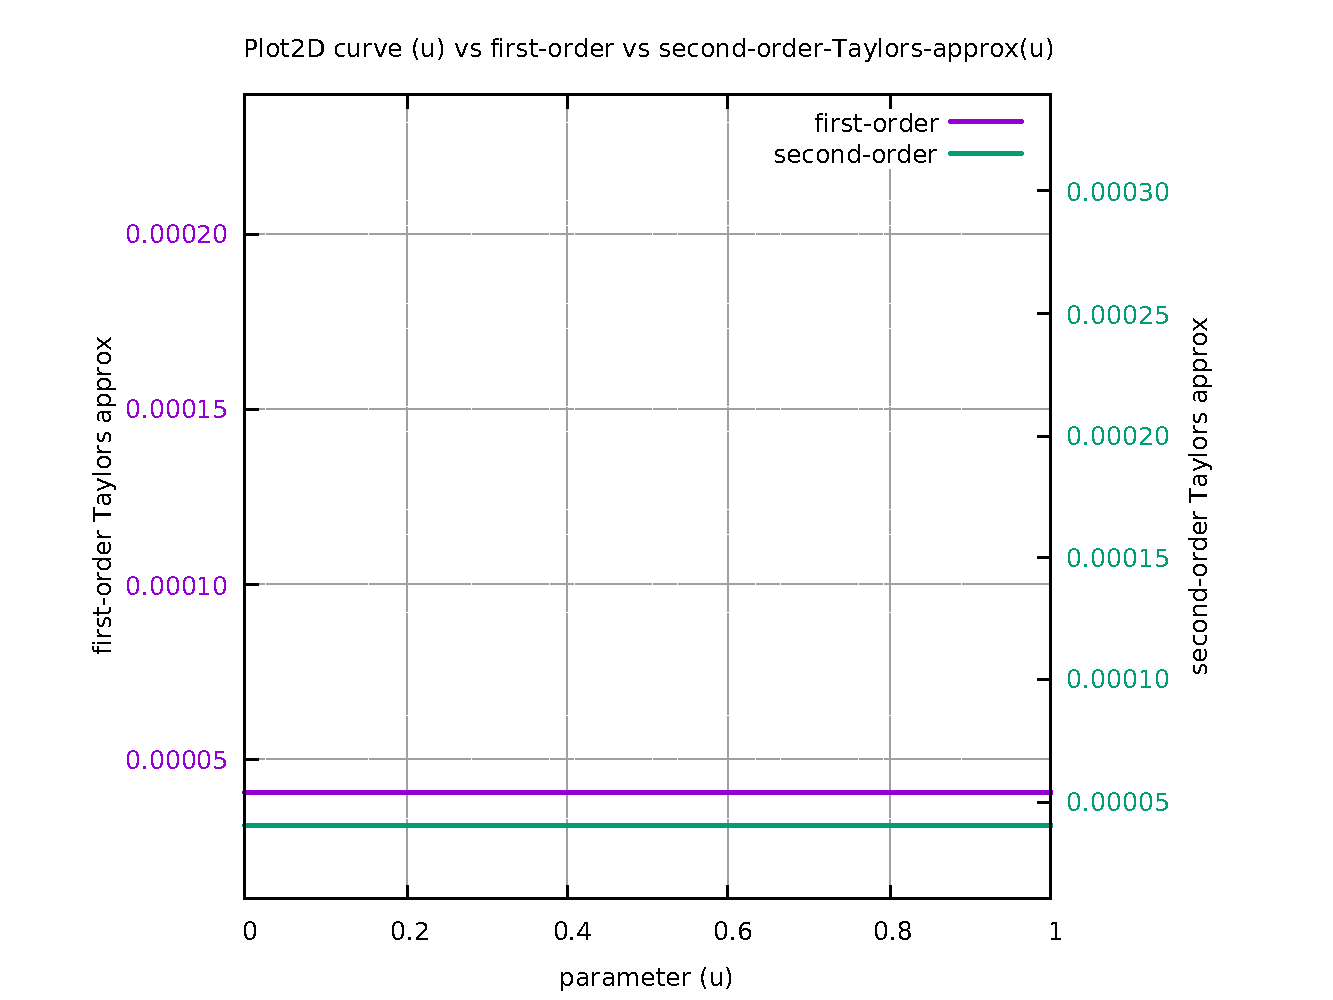
\includegraphics[width=1.00\textwidth]{Chap4/appendix/app-Circle/plots/07-img-Circle-Separation-First-and-Second-Order-Taylors-Approx.pdf}
\end{figure}


\begin{figure}
	\caption     {Circle Separation SAL and SCL}
	\label{08-img-Circle-Separation-SAL-and-SCL.pdf}
	%%	\centering
	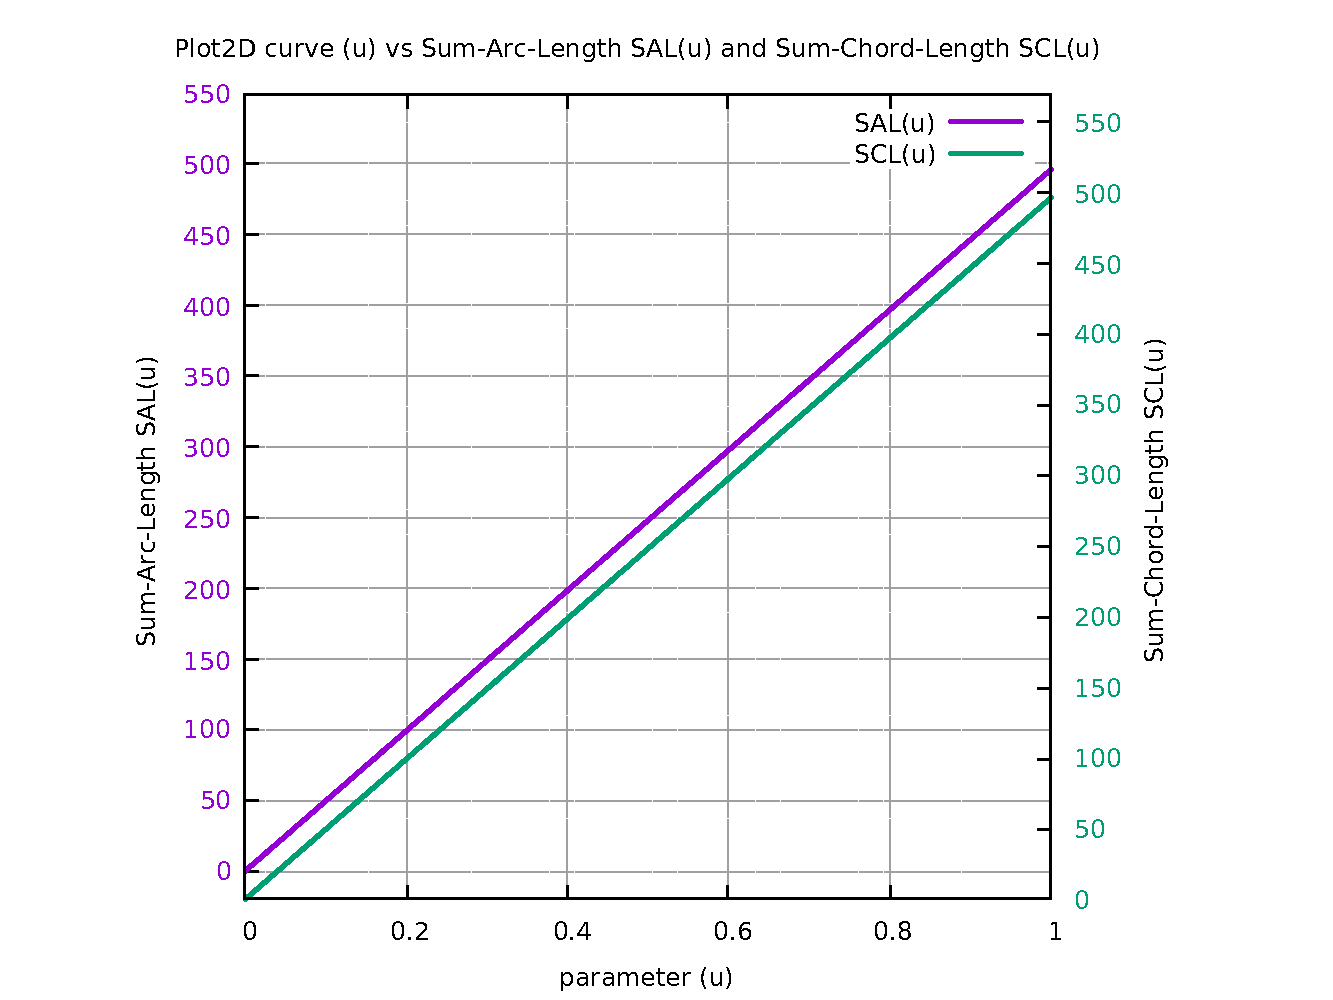
\includegraphics[width=1.00\textwidth]{Chap4/appendix/app-Circle/plots/08-img-Circle-Separation-SAL-and-SCL.pdf}
\end{figure}

%% ==================================================
\clearpage
\pagebreak

\begin{figure}
	\caption     {Circle Chord-error in close view 2 scales}
	\label{09-img-Circle-Chord-error-in-close-view-2-scales.pdf}
	%%	\centering
	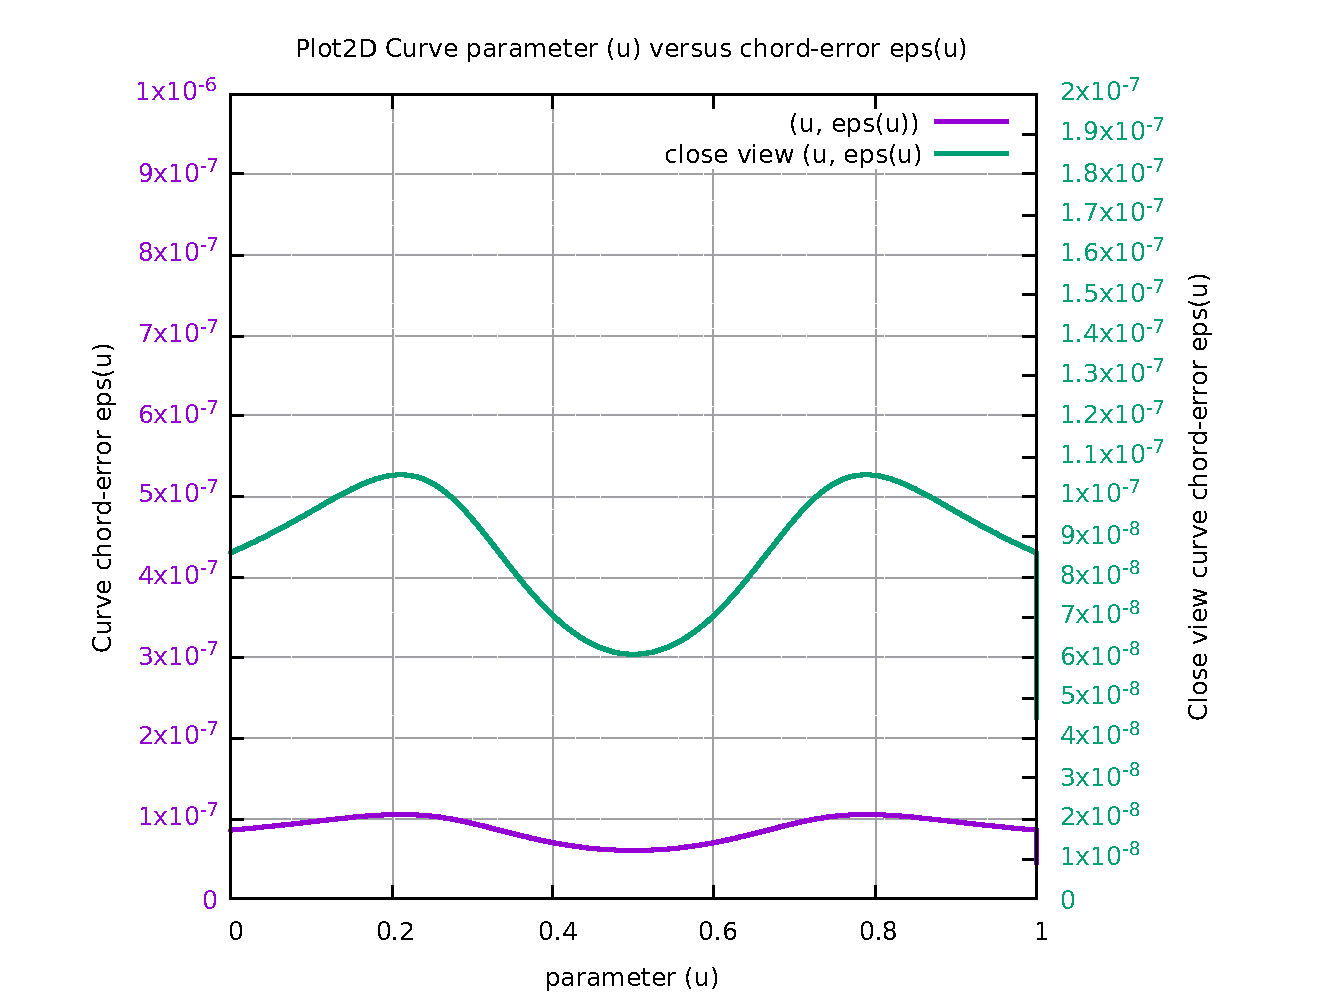
\includegraphics[width=1.00\textwidth]{Chap4/appendix/app-Circle/plots/09-img-Circle-Chord-error-in-close-view-2-scales.pdf}
\end{figure}


\begin{figure}
	\caption     {Circle Four Components Feedrate Limit}
	\label{10-img-Circle-Four-Components-Feedrate-Limit.pdf}
	%%	\centering
	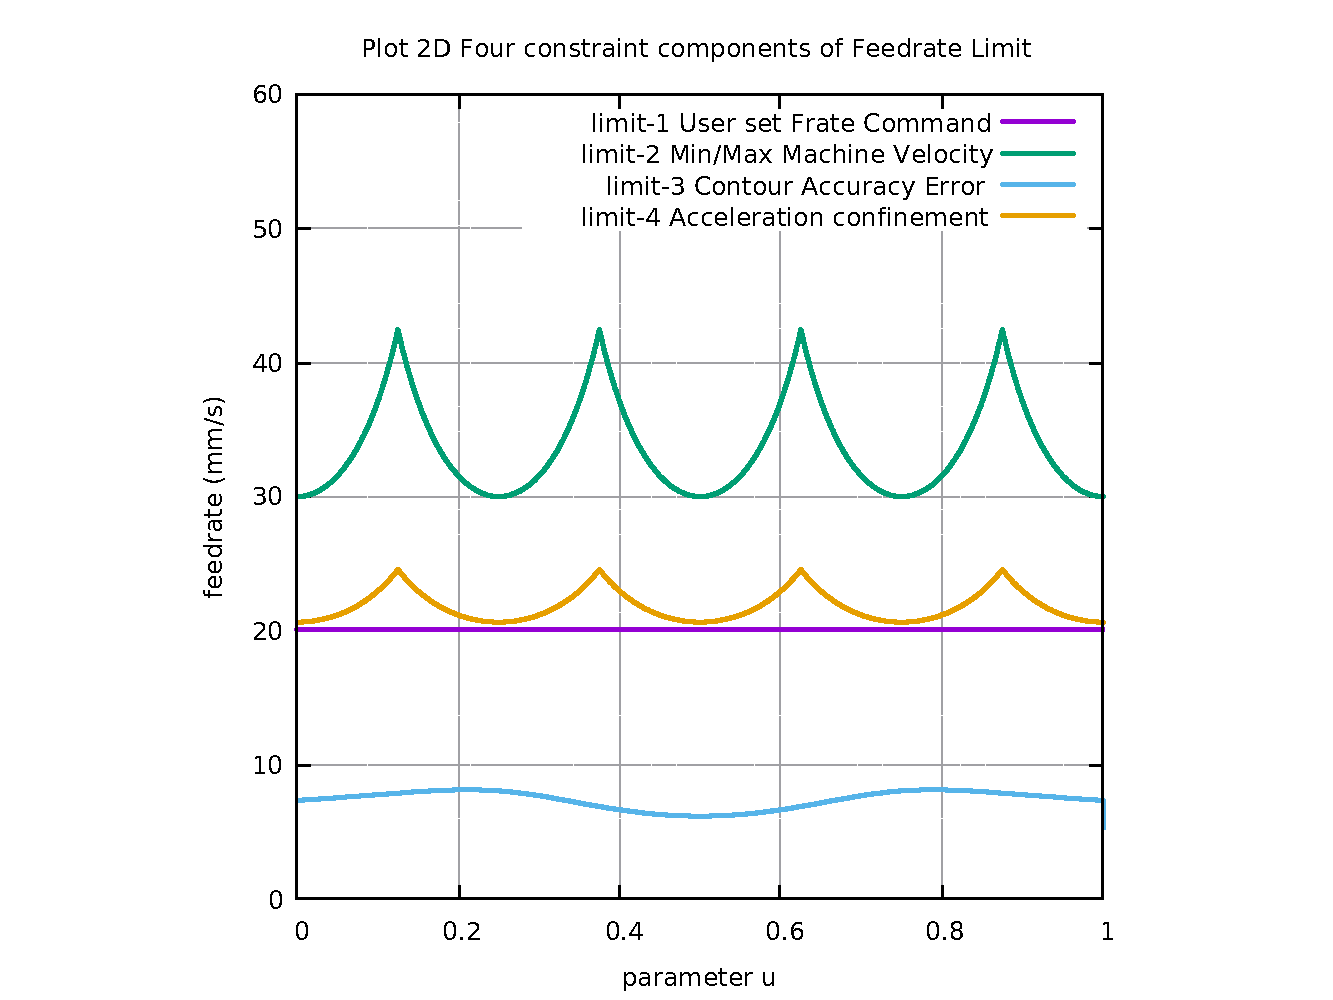
\includegraphics[width=1.00\textwidth]{Chap4/appendix/app-Circle/plots/10-img-Circle-Four-Components-Feedrate-Limit.pdf}
\end{figure}

%% ==================================================
\clearpage
\pagebreak

\begin{figure}
	\caption     {Circle FrateCommand FrateLimit and Curr-Frate}
	\label{11-img-Circle-FrateCommand-FrateLimit-and-Curr-Frate.pdf}
	%%	\centering
	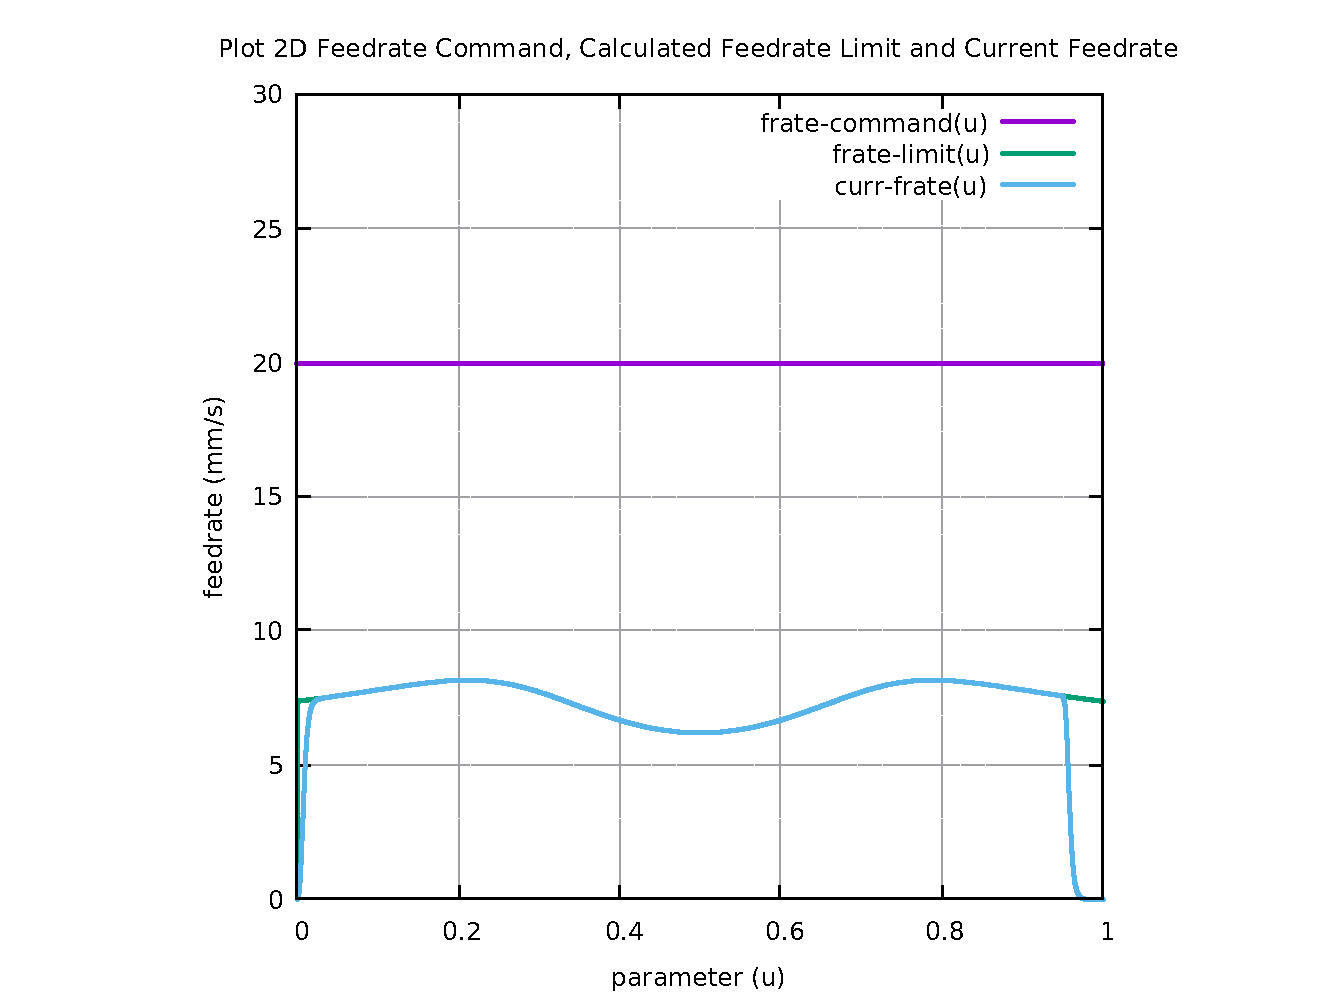
\includegraphics[width=1.00\textwidth]{Chap4/appendix/app-Circle/plots/11-img-Circle-FrateCommand-FrateLimit-and-Curr-Frate.pdf}
\end{figure}


\begin{figure}
	\caption     {Circle FeedRateLimit minus CurrFeedRate}
	\label{12-img-Circle-FeedRateLimit-minus-CurrFeedRate.pdf}
	%%	\centering
	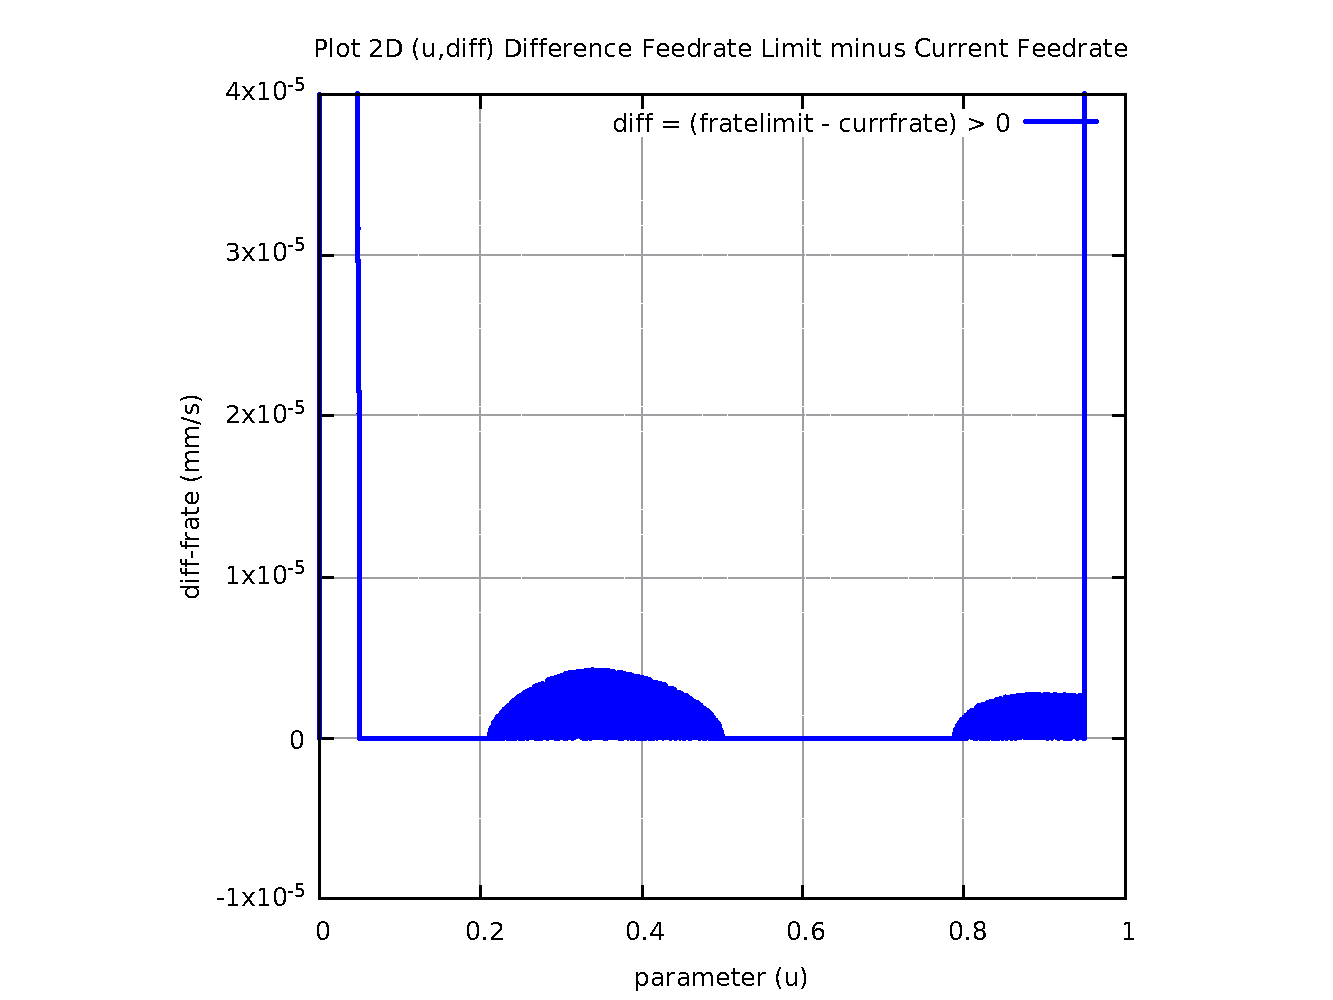
\includegraphics[width=1.00\textwidth]{Chap4/appendix/app-Circle/plots/12-img-Circle-FeedRateLimit-minus-CurrFeedRate.pdf}
\end{figure}

%% ==================================================
\clearpage
\pagebreak

\begin{figure}
	\caption     {Circle FC20-Nominal X and Y Feedrate Profiles}
	\label{13-img-Circle-FC20-Nominal-X-and-Y-Feedrate-Profiles.pdf}
	%%	\centering
	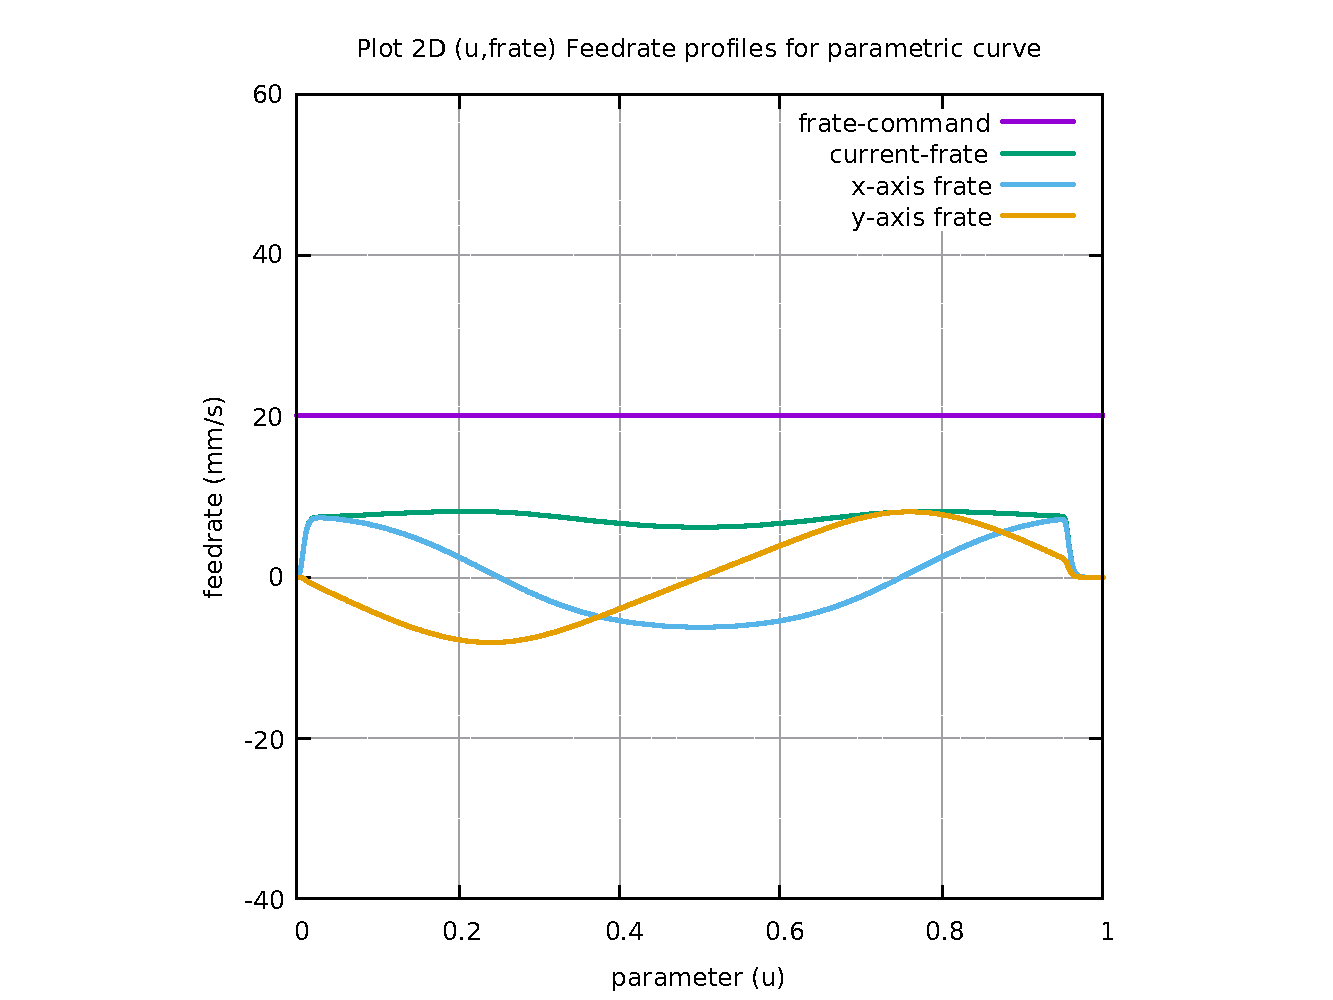
\includegraphics[width=1.00\textwidth]{Chap4/appendix/app-Circle/plots/13-img-Circle-FC20-Nominal-X-and-Y-Feedrate-Profiles.pdf}
\end{figure}


\begin{figure}
	\caption     {Circle FC20 Nominal Tangential Acceleration}
	\label{14-img-Circle-FC20-Nominal-Tangential-Acceleration.pdf}
	%%	\centering
	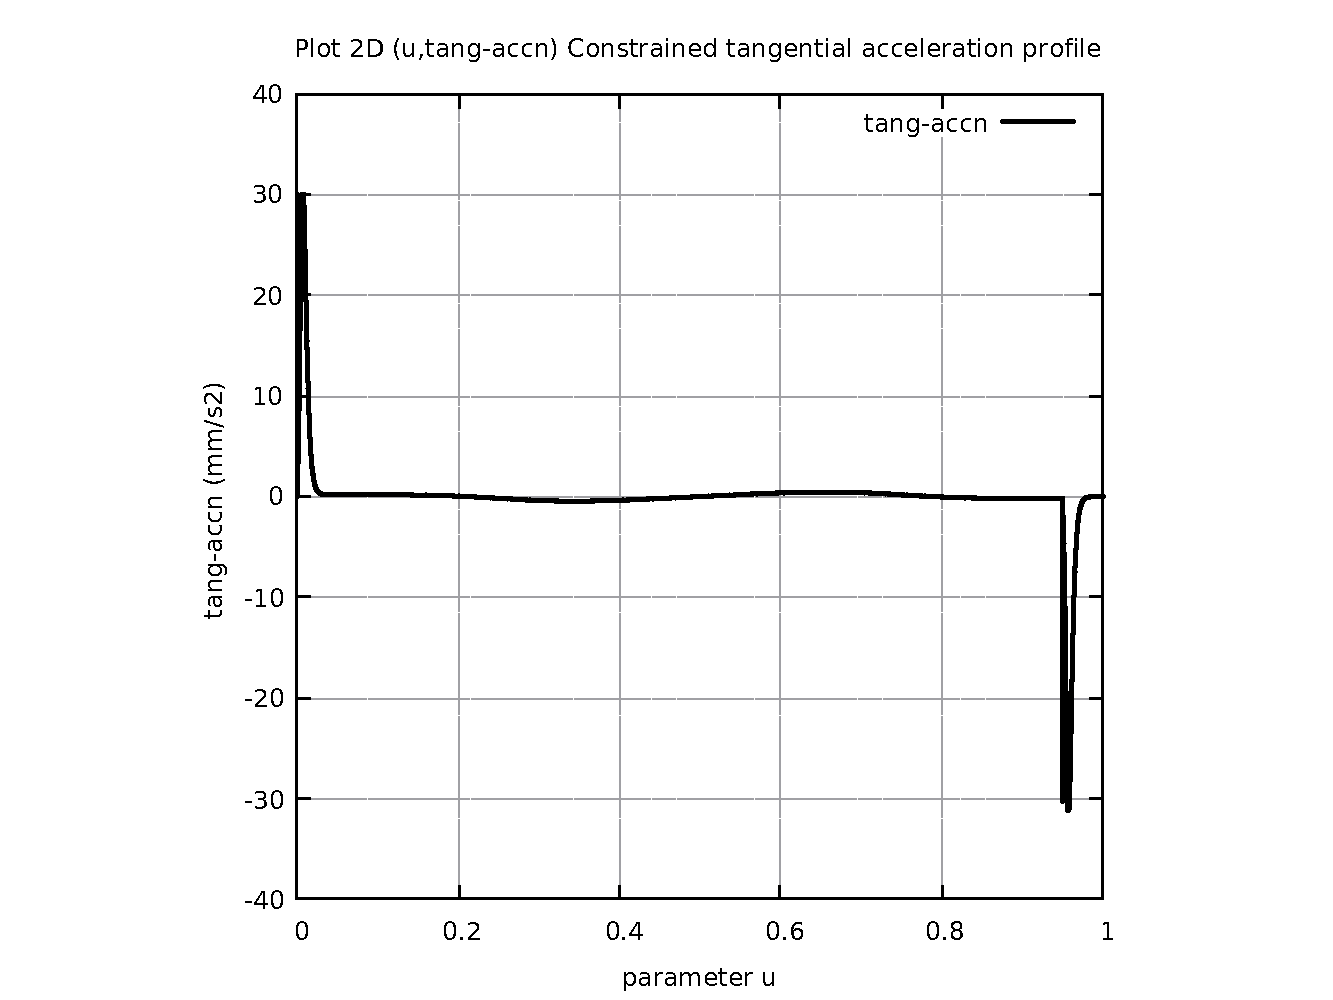
\includegraphics[width=1.00\textwidth]{Chap4/appendix/app-Circle/plots/14-img-Circle-FC20-Nominal-Tangential-Acceleration.pdf}
\end{figure}

%% ==================================================
\clearpage
\pagebreak

\begin{figure}
	\caption     {Circle FC20 Nominal Rising S-Curve Profile}
	\label{15-img-Circle-FC20-Nominal-Rising-S-Curve-Profile.pdf}
	%%	\centering
	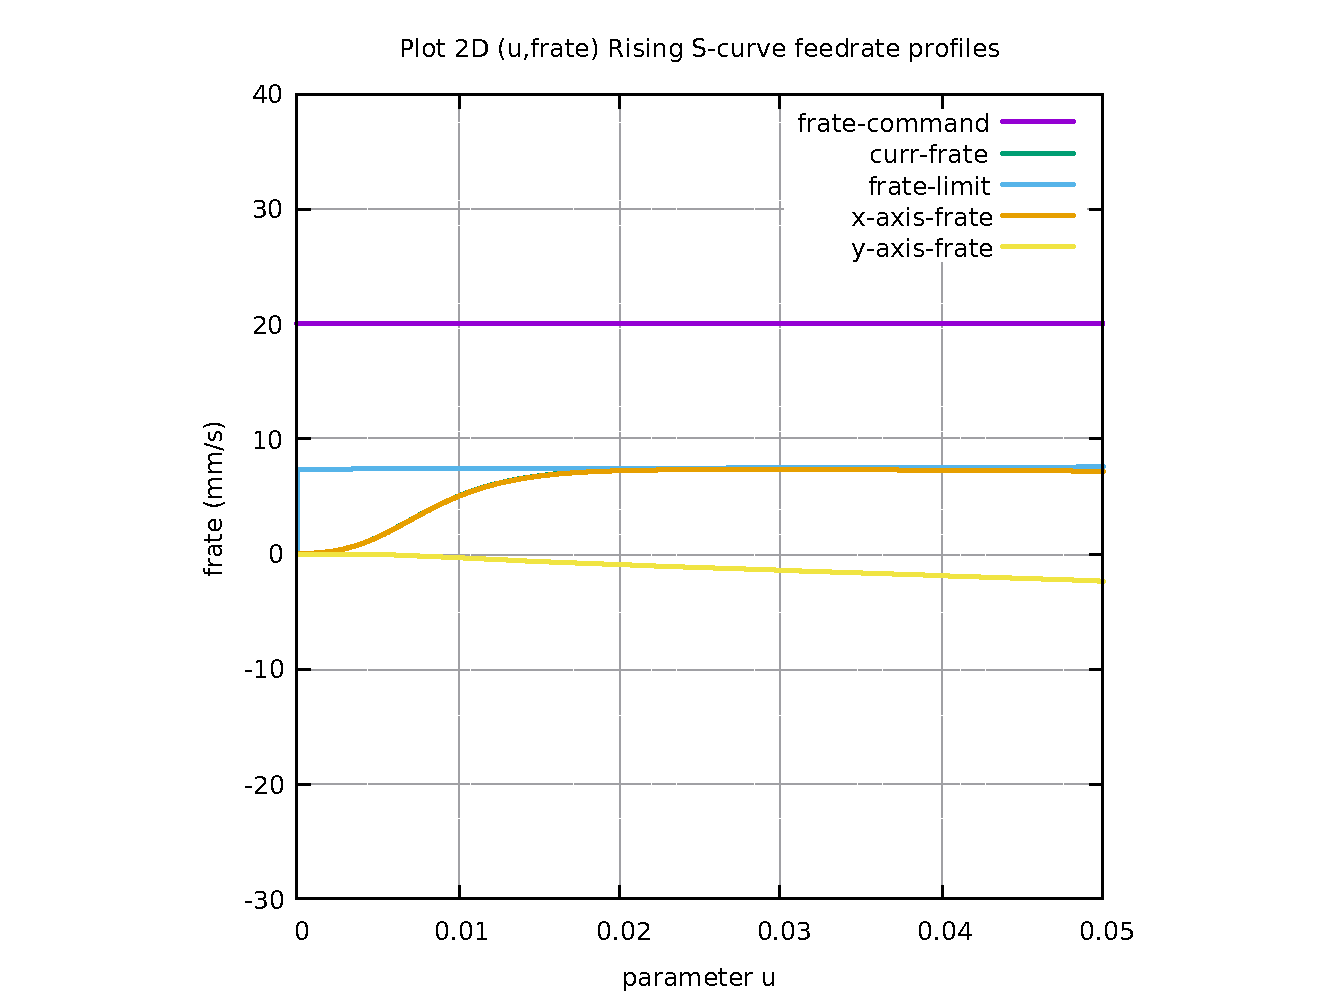
\includegraphics[width=1.00\textwidth]{Chap4/appendix/app-Circle/plots/15-img-Circle-FC20-Nominal-Rising-S-Curve-Profile.pdf}
\end{figure}


\begin{figure}
	\caption     {Circle FC20 Nominal Falling S-Curve Profile}
	\label{16-img-Circle-FC20-Nominal-Falling-S-Curve-Profile.pdf}
	%%	\centering
	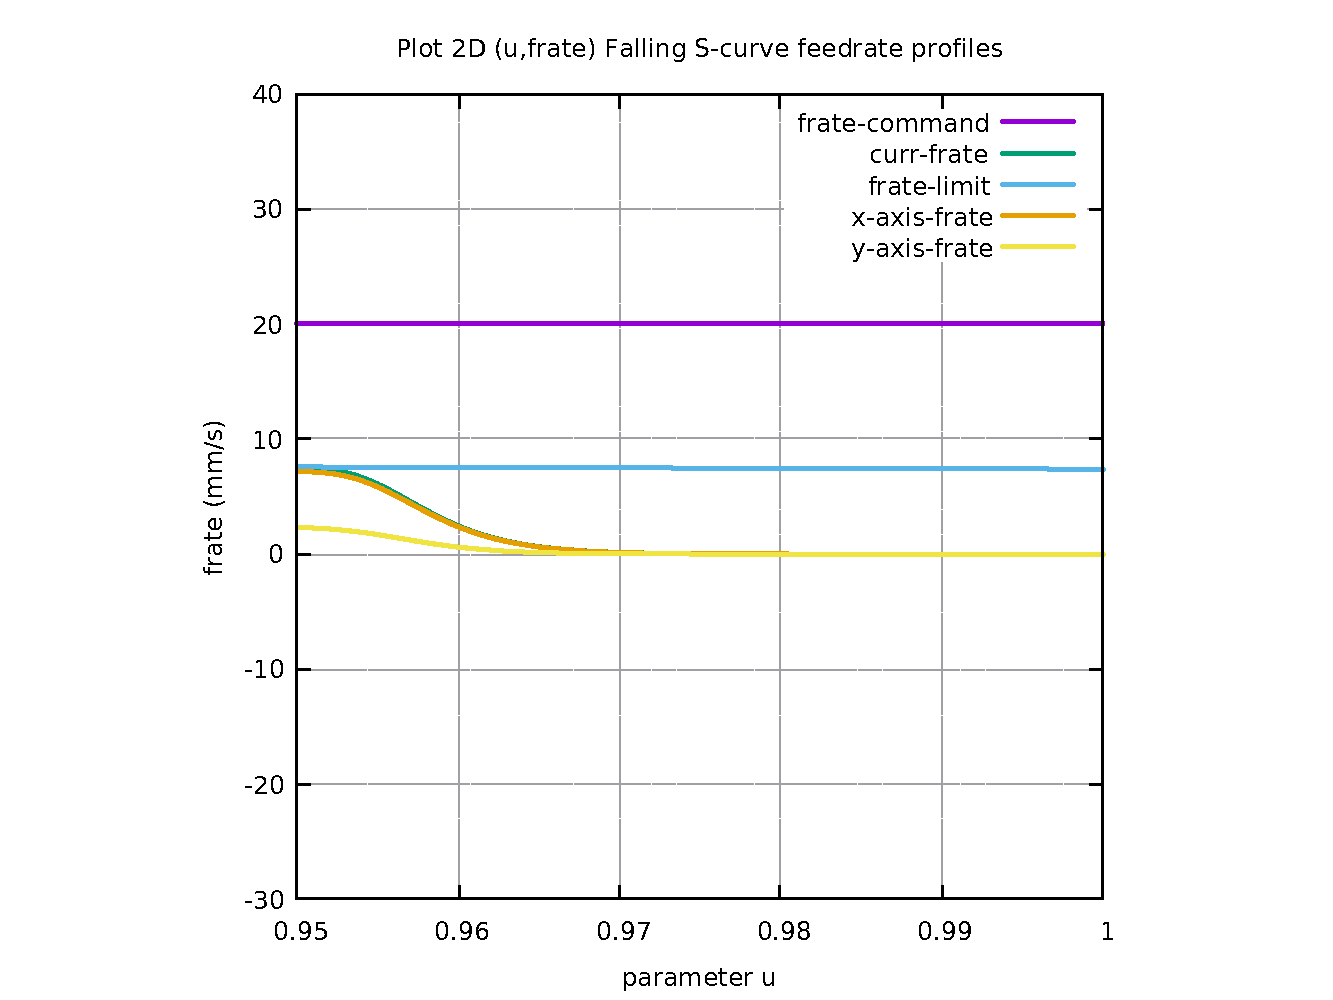
\includegraphics[width=1.00\textwidth]{Chap4/appendix/app-Circle/plots/16-img-Circle-FC20-Nominal-Falling-S-Curve-Profile.pdf}
\end{figure}

%% ==================================================
\clearpage
\pagebreak

\begin{figure}
	\caption     {Circle FC10 Colored Feedrate Profile data ngcode}
	\label{17-img-Circle-FC10-Colored-Feedrate-Profile-data_ngcode.png}
	%%	\centering
	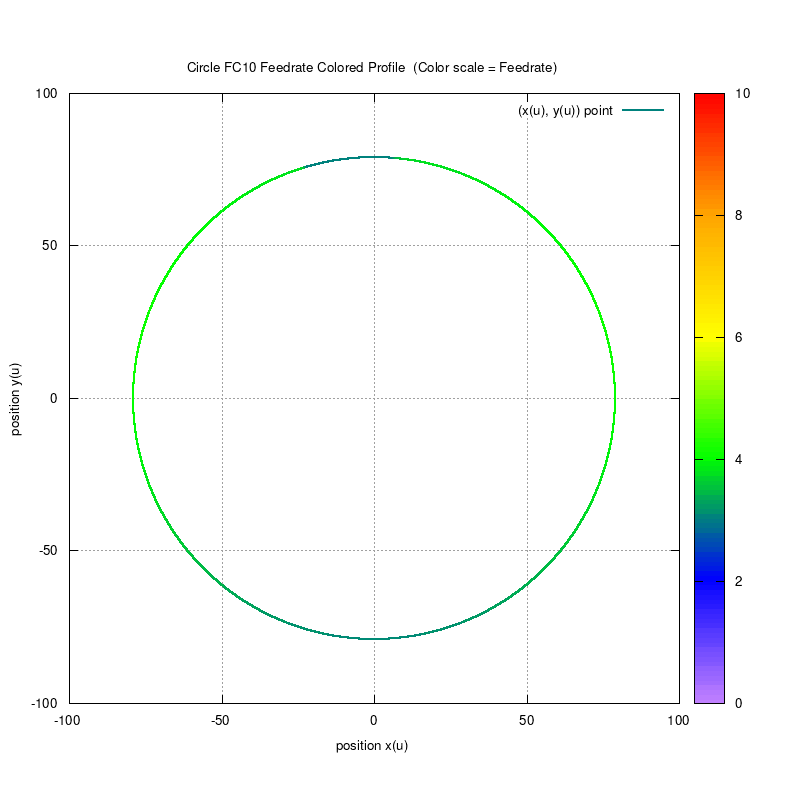
\includegraphics[width=0.75\textwidth]{Chap4/appendix/app-Circle/plots/17-img-Circle-FC10-Colored-Feedrate-Profile-data_ngcode.png}
\end{figure}


\begin{figure}
	\caption     {Circle FC20 Colored Feedrate Profile data ngcode}
	\label{18-img-Circle-FC20-Colored-Feedrate-Profile-data_ngcode.png}
	%%	\centering
	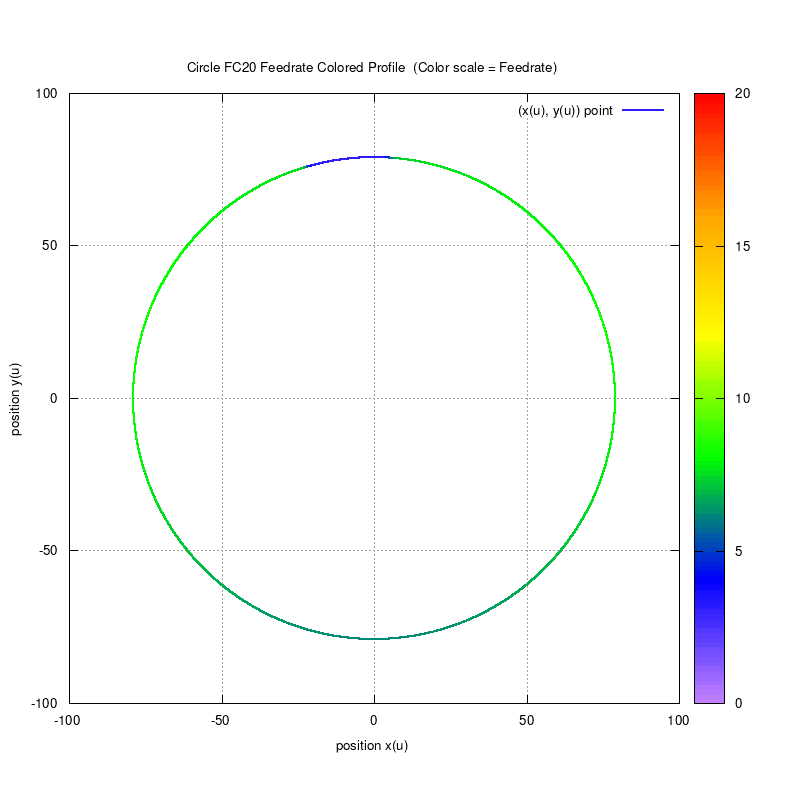
\includegraphics[width=0.75\textwidth]{Chap4/appendix/app-Circle/plots/18-img-Circle-FC20-Colored-Feedrate-Profile-data_ngcode.png}
\end{figure}

%% ==================================================
\clearpage
\pagebreak

\begin{figure}
	\caption     {Circle FC30 Colored Feedrate Profile data ngcode}
	\label{19-img-Circle-FC30-Colored-Feedrate-Profile-data_ngcode.png}
	%%	\centering
	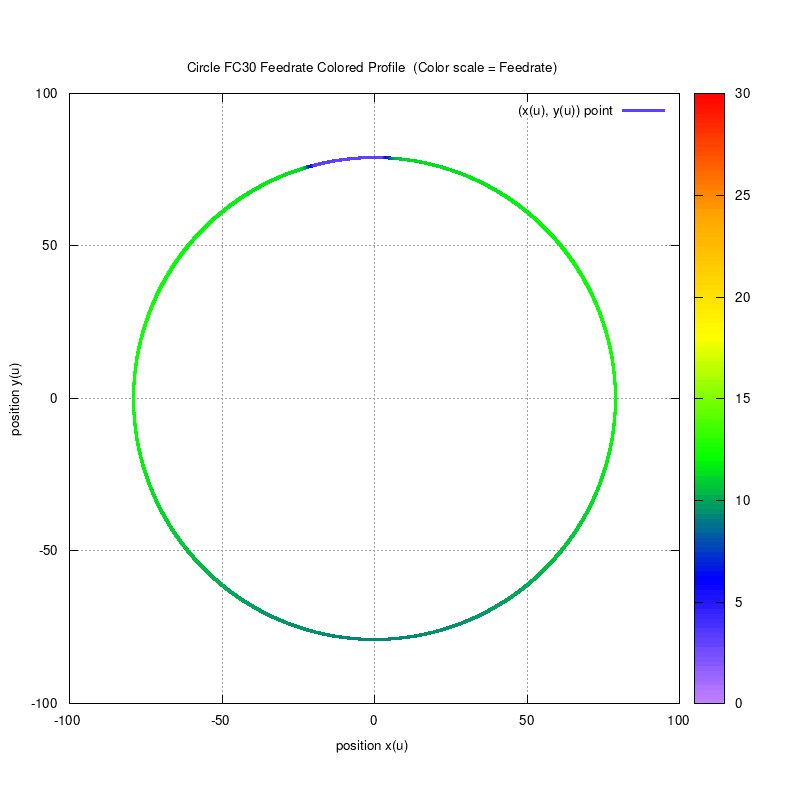
\includegraphics[width=0.75\textwidth]{Chap4/appendix/app-Circle/plots/19-img-Circle-FC30-Colored-Feedrate-Profile-data_ngcode.png}
\end{figure}


\begin{figure}
	\caption     {Circle FC40 Colored Feedrate Profile data ngcode}
	\label{20-img-Circle-FC40-Colored-Feedrate-Profile-data_ngcode.png}
	%%	\centering
	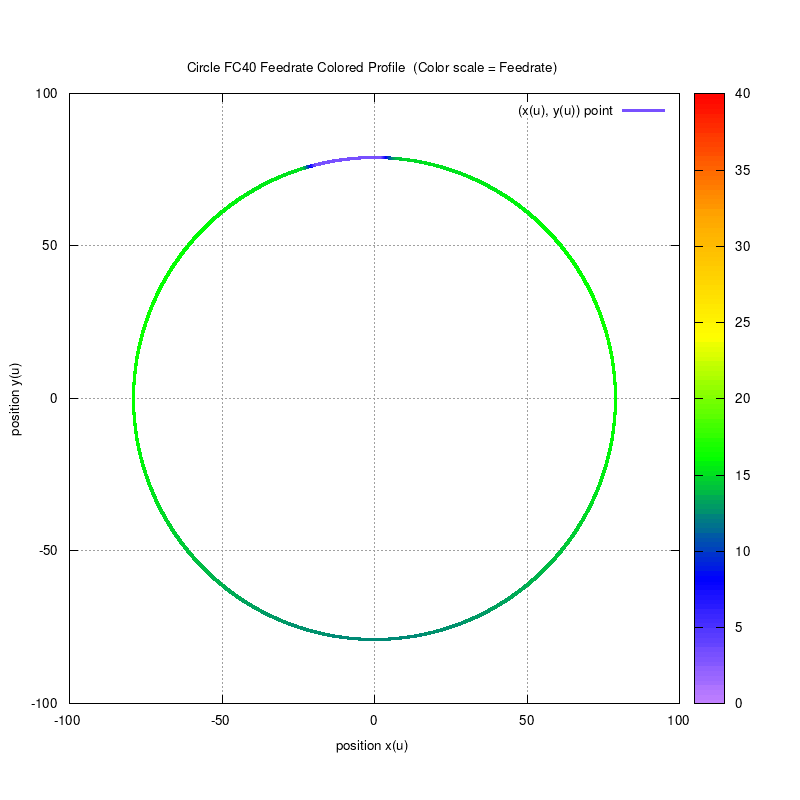
\includegraphics[width=0.75\textwidth]{Chap4/appendix/app-Circle/plots/20-img-Circle-FC40-Colored-Feedrate-Profile-data_ngcode.png}
\end{figure}

%% ==================================================
\clearpage
\pagebreak

\begin{figure}
	\caption     {Circle FC10 Tangential Acceleration}
	\label{21-img-Circle-FC10-Tangential-Acceleration.pdf}
	%%	\centering
	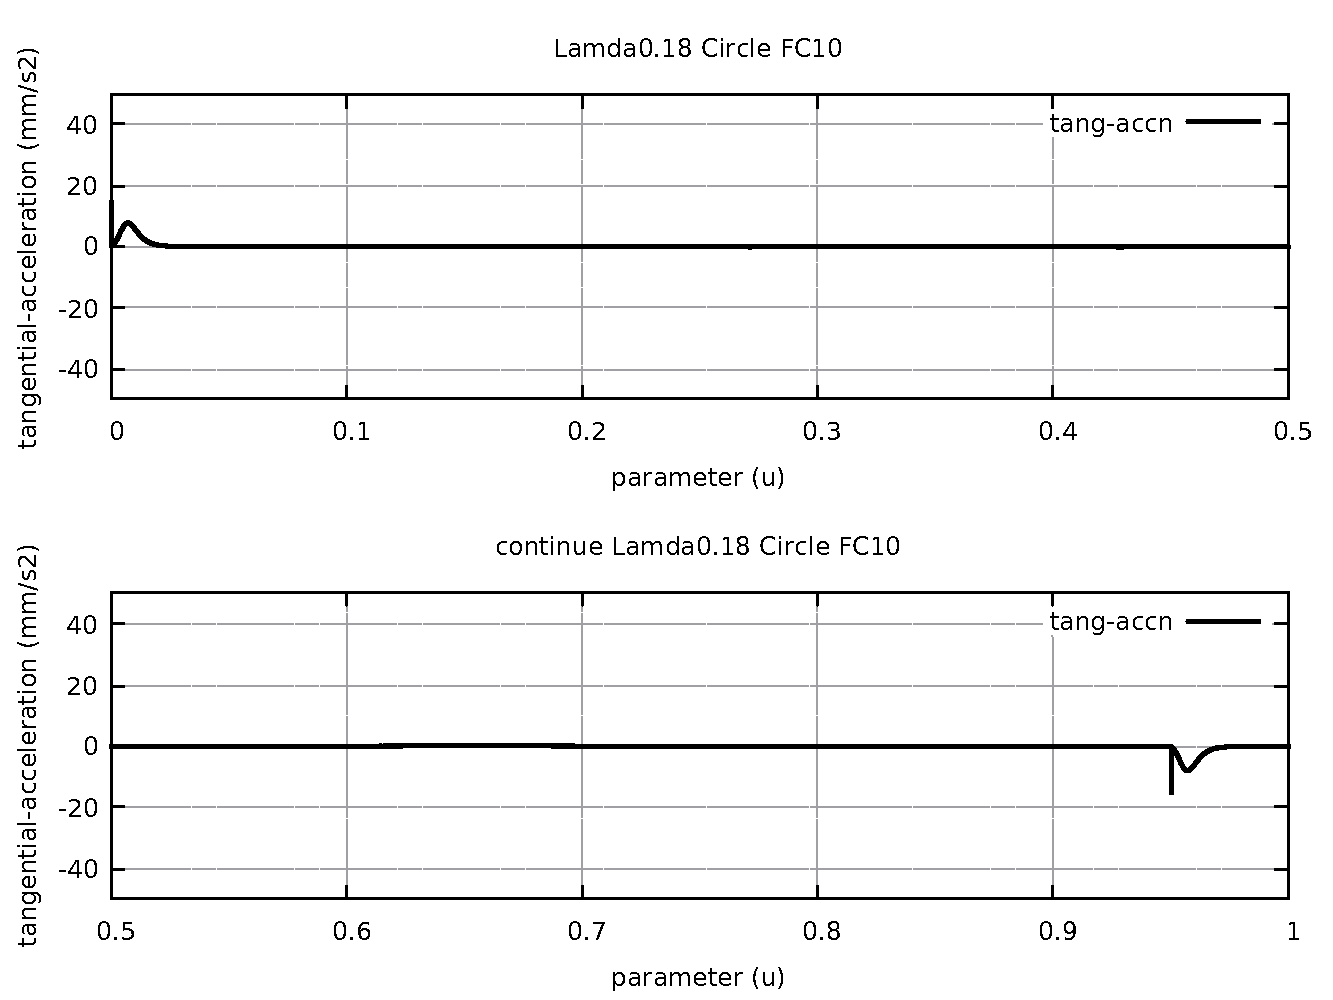
\includegraphics[width=1.00\textwidth]{Chap4/appendix/app-Circle/plots/21-img-Circle-FC10-Tangential-Acceleration.pdf}
\end{figure}


\begin{figure}
	\caption     {Circle FC20 Tangential Acceleration}
	\label{22-img-Circle-FC20-Tangential-Acceleration.pdf}
	%%	\centering
	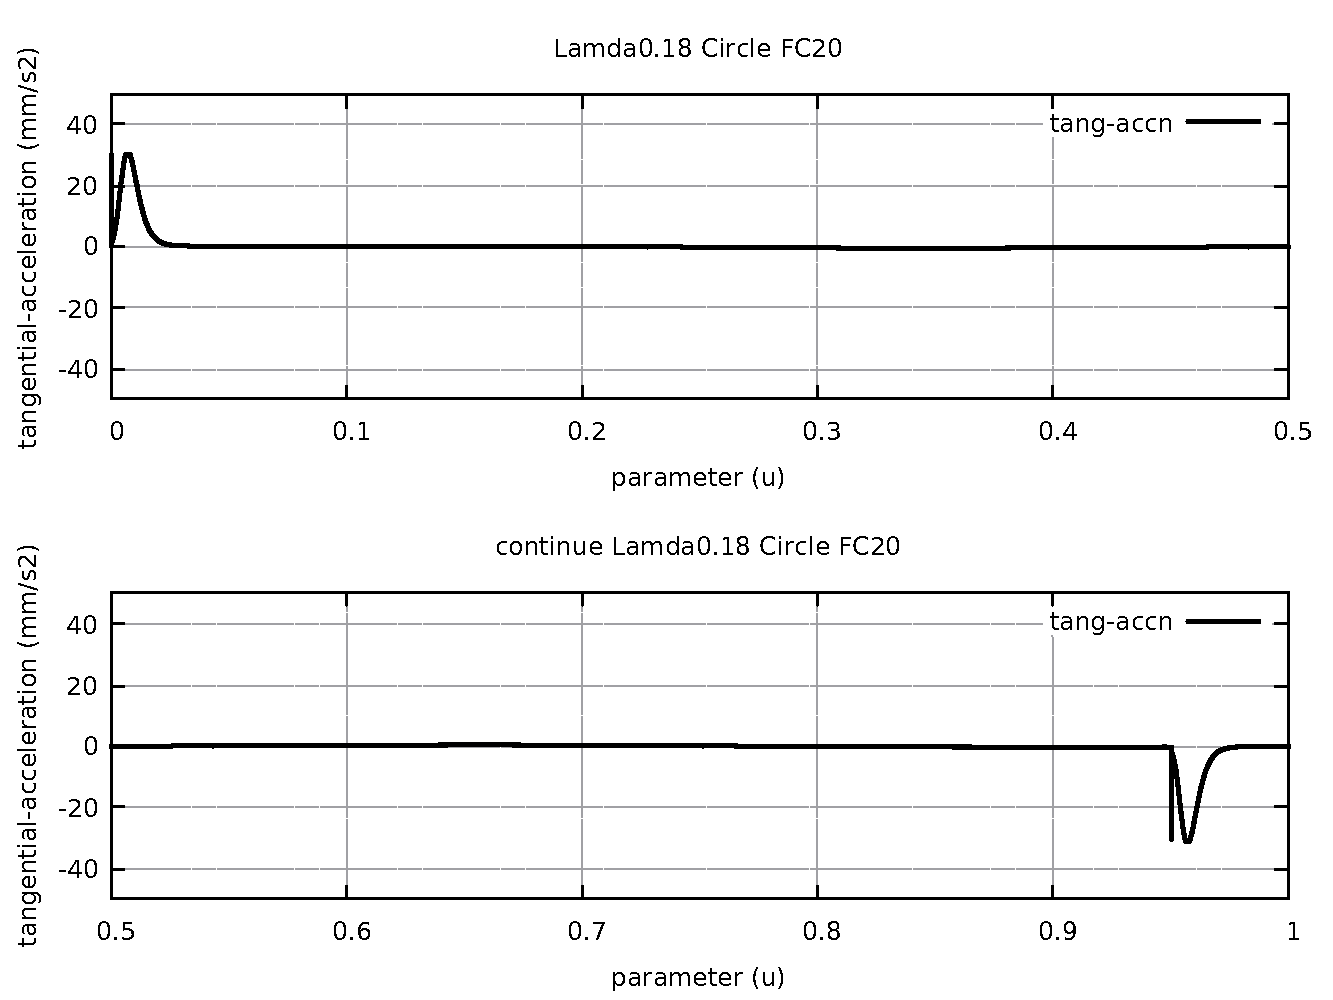
\includegraphics[width=1.00\textwidth]{Chap4/appendix/app-Circle/plots/22-img-Circle-FC20-Tangential-Acceleration.pdf}
\end{figure}

%% ==================================================
\clearpage
\pagebreak

\begin{figure}
	\caption     {Circle FC30 Tangential Acceleration}
	\label{23-img-Circle-FC30-Tangential-Acceleration.pdf}
	%%	\centering
	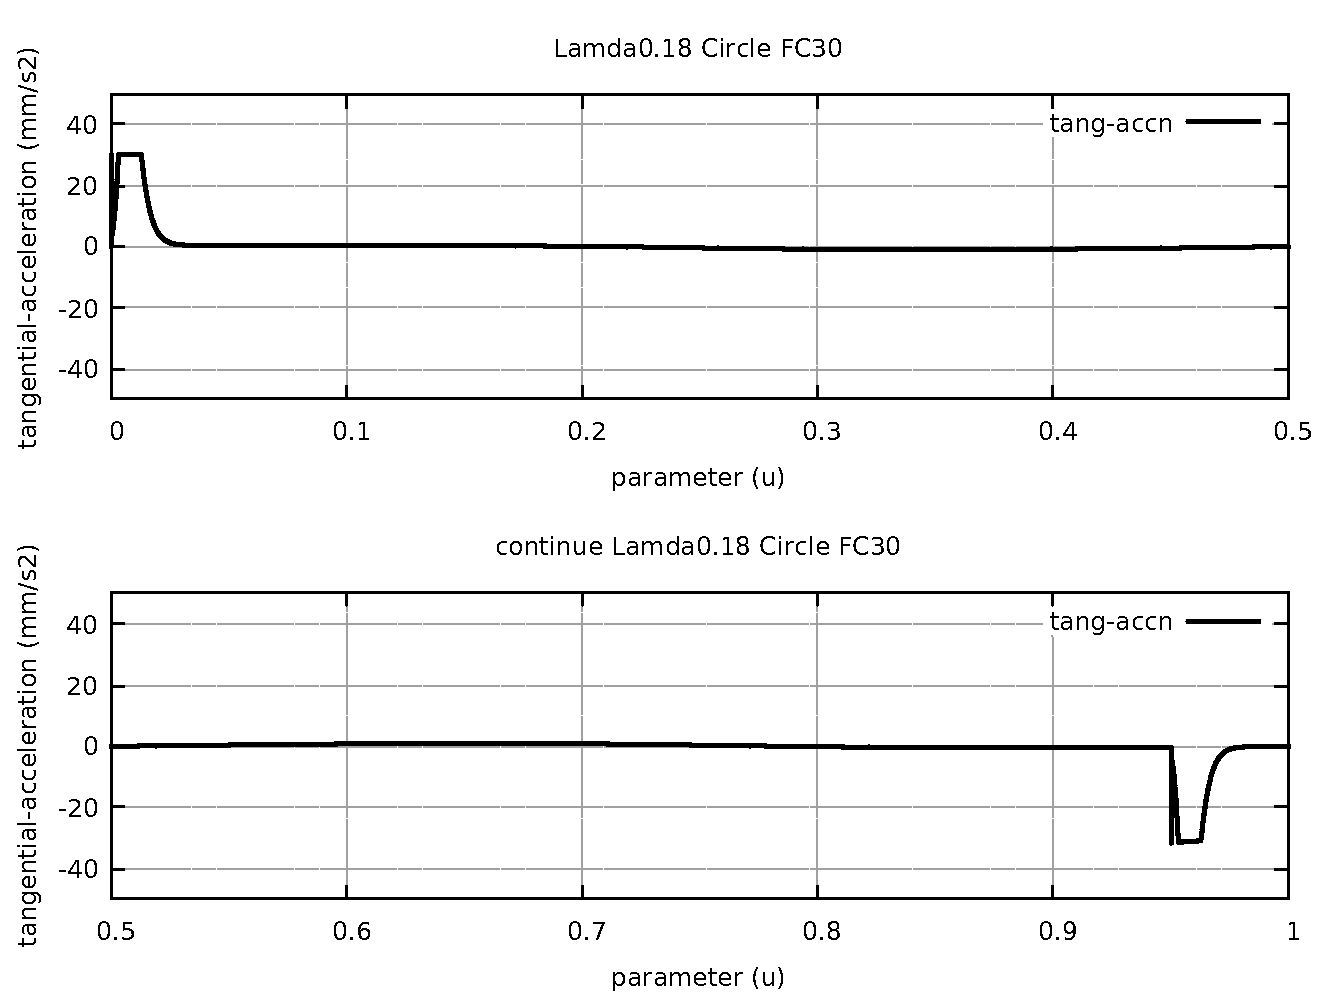
\includegraphics[width=1.00\textwidth]{Chap4/appendix/app-Circle/plots/23-img-Circle-FC30-Tangential-Acceleration.pdf}
\end{figure}


\begin{figure}
	\caption     {Circle FC40 Tangential Acceleration}
	\label{24-img-Circle-FC40-Tangential-Acceleration.pdf}
	%%	\centering
	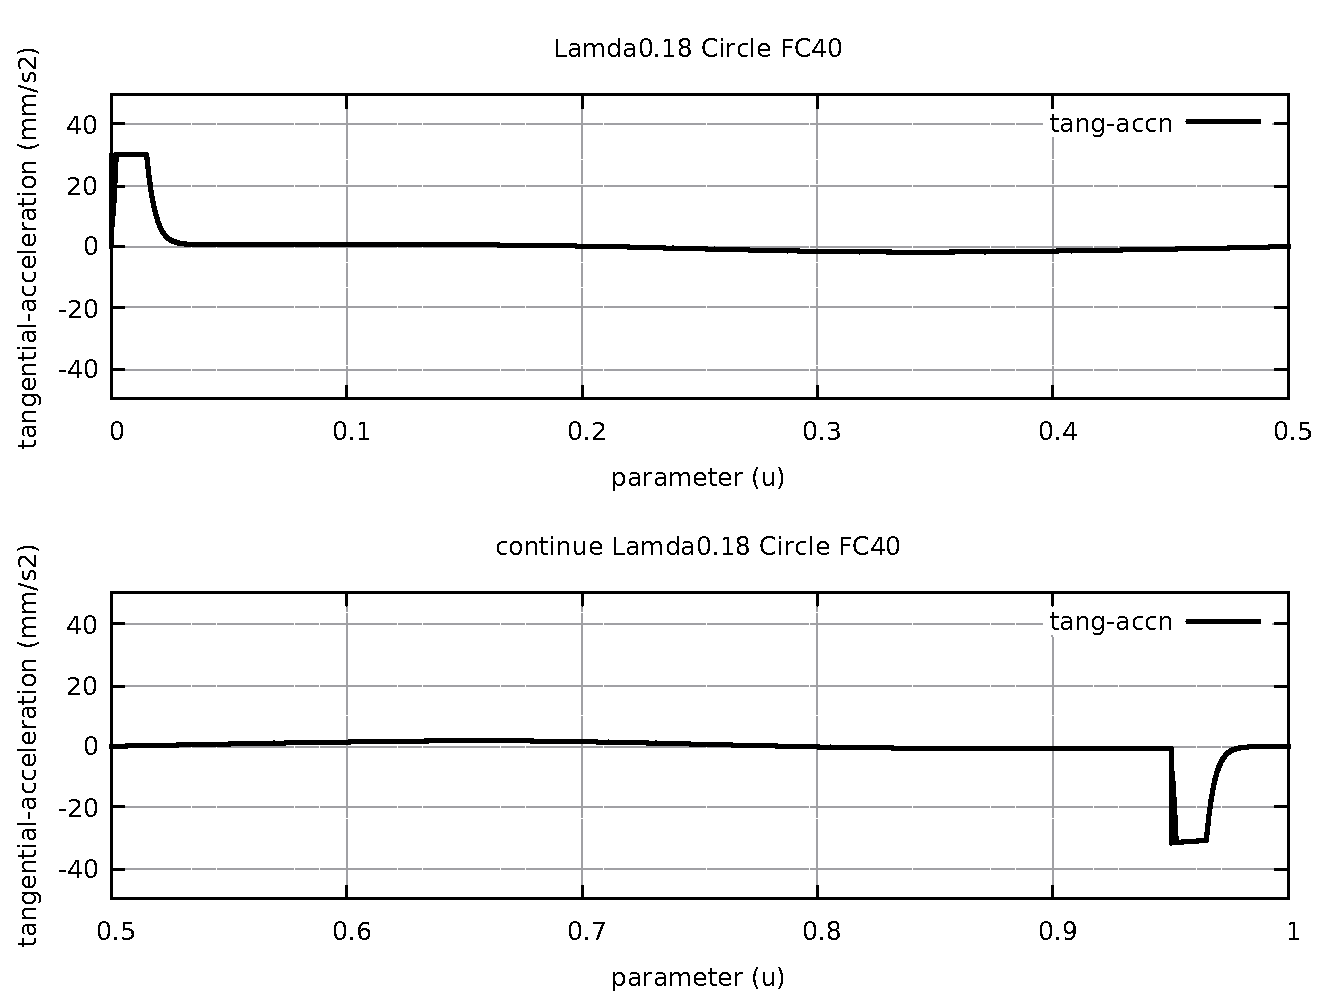
\includegraphics[width=1.00\textwidth]{Chap4/appendix/app-Circle/plots/24-img-Circle-FC40-Tangential-Acceleration.pdf}
\end{figure}

%% ==================================================
\clearpage
\pagebreak

\begin{figure}
	\caption     {Circle FC20 Nominal Separation NAL and NCL}
	\label{25-img-Circle-FC20-Nominal-Separation-NAL-and-NCL.pdf}
	%%	\centering
	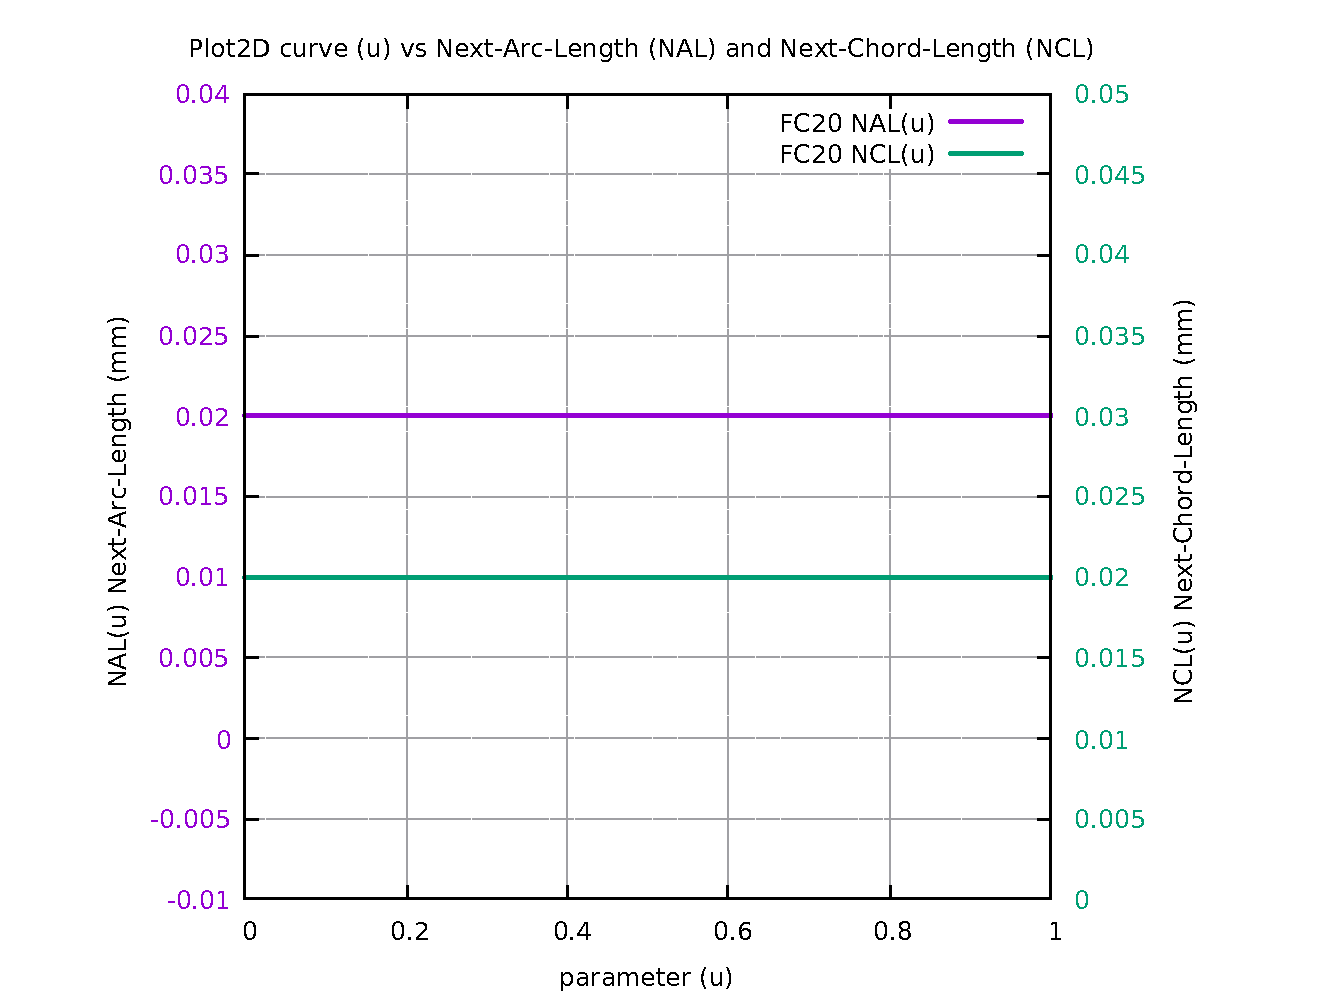
\includegraphics[width=1.00\textwidth]{Chap4/appendix/app-Circle/plots/25-img-Circle-FC20-Nominal-Separation-NAL-and-NCL.pdf}
\end{figure}


\begin{figure}
	\caption     {Circle Difference SAL minus SCL for FC10 FC20 FC30 FC40}
	\label{26-img-Circle-Difference-SAL-minus-SCL-for-FC10-FC20-FC30-FC40.pdf}
	%%	\centering
	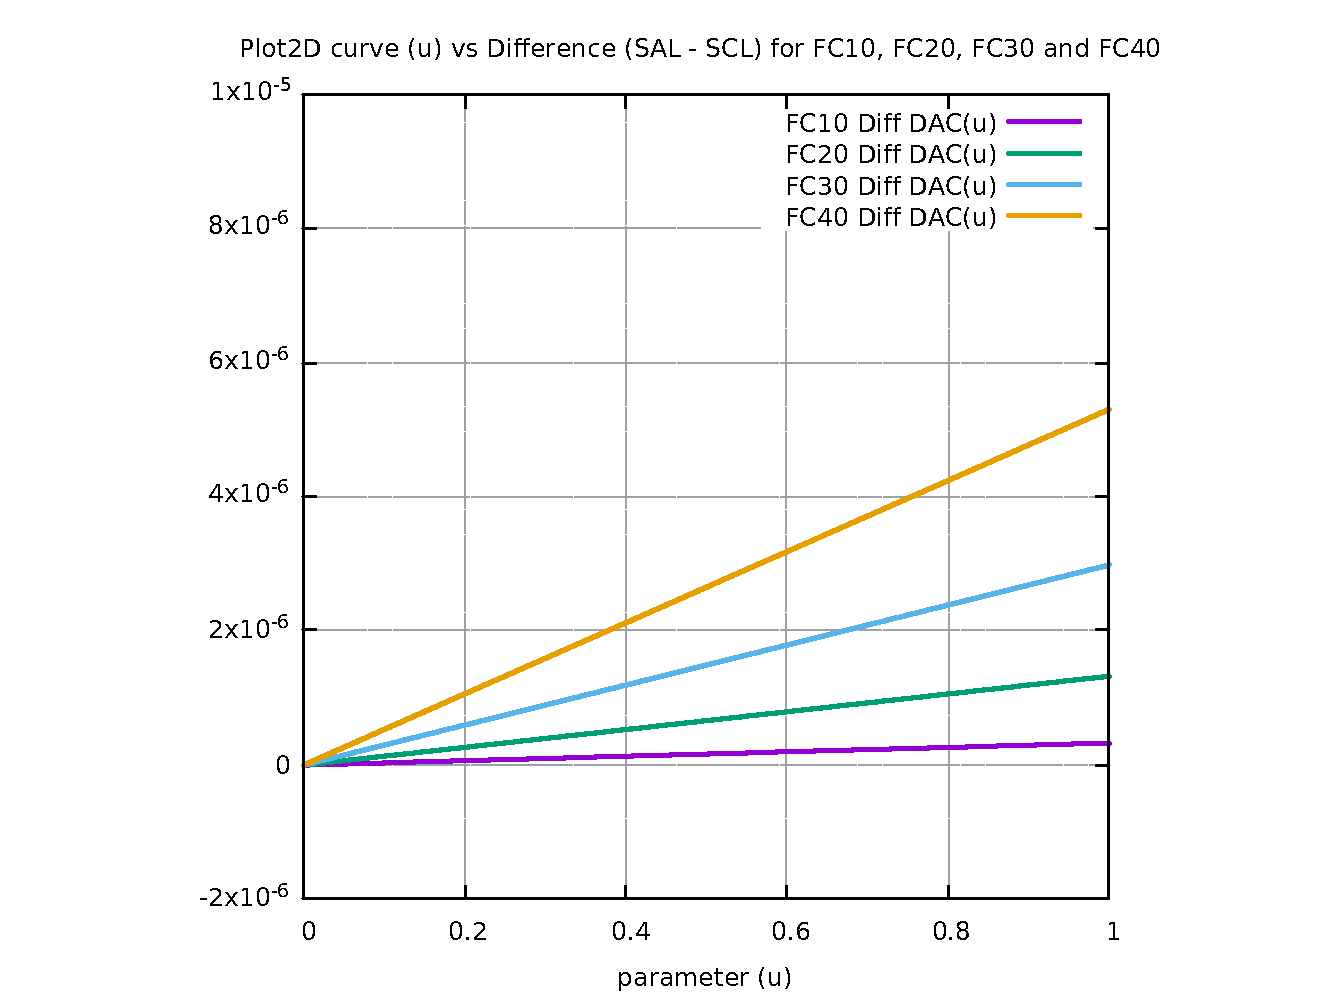
\includegraphics[width=1.00\textwidth]{Chap4/appendix/app-Circle/plots/26-img-Circle-Difference-SAL-minus-SCL-for-FC10-FC20-FC30-FC40.pdf}
\end{figure}


%% ==================================================
\clearpage
\pagebreak

\begin{figure}
	\caption     {Circle FC10 FrateCmd CurrFrate X-Frate Y-Frate}
	\label{27-img-Circle-FC10-FrateCmd-CurrFrate-X-Frate-Y-Frate.pdf}
	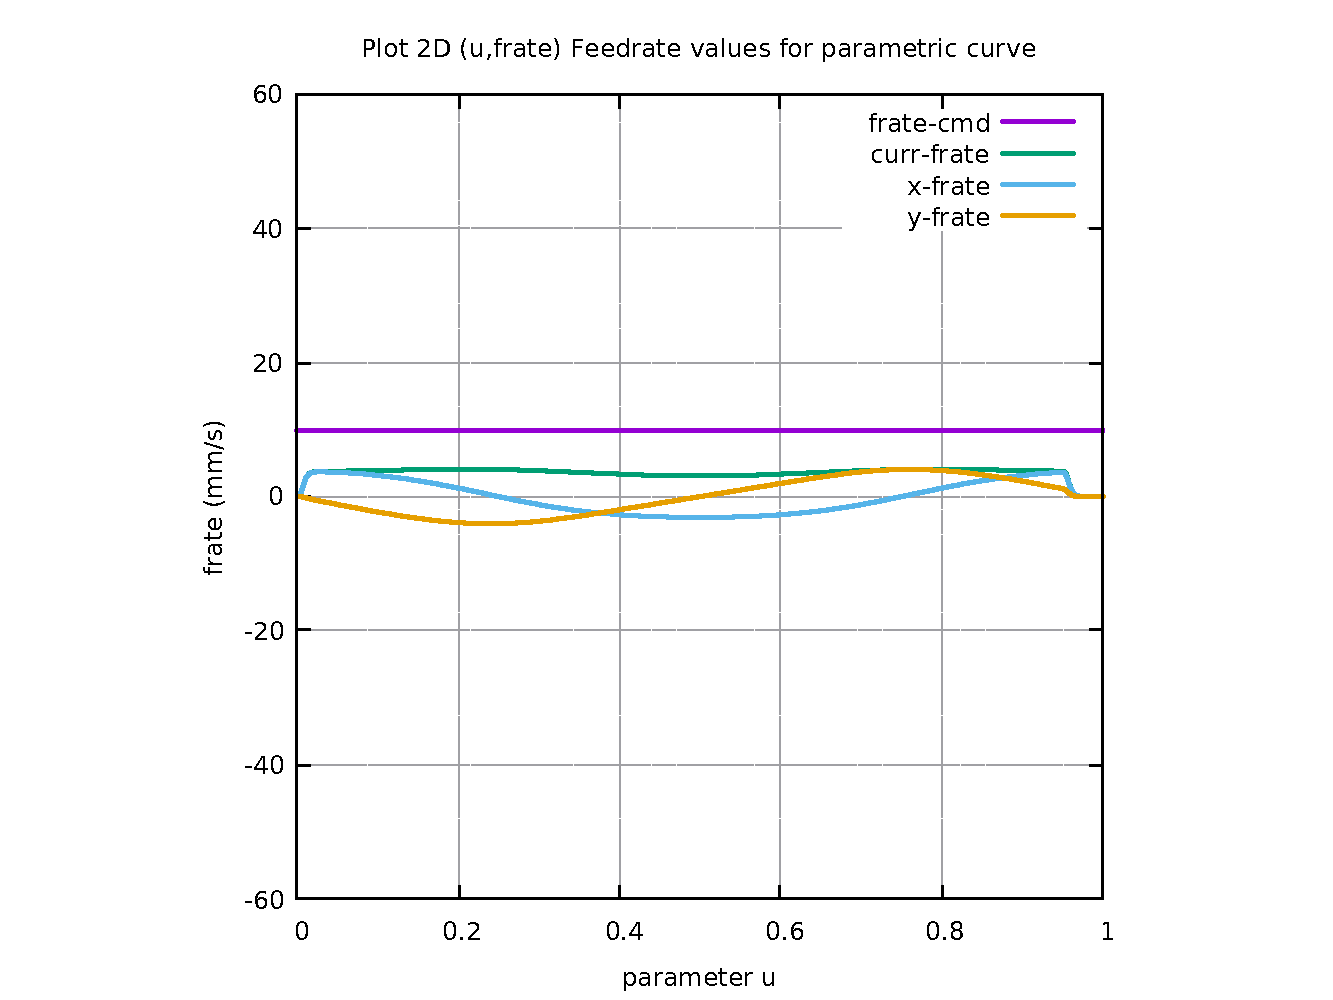
\includegraphics[width=1.00\textwidth]{Chap4/appendix/app-Circle/plots/27-img-Circle-FC10-FrateCmd-CurrFrate-X-Frate-Y-Frate.pdf}
\end{figure}


\begin{figure}
	\caption     {Circle FC20 FrateCmd CurrFrate X-Frate Y-Frate}
	\label{28-img-Circle-FC20-FrateCmd-CurrFrate-X-Frate-Y-Frate.pdf}
	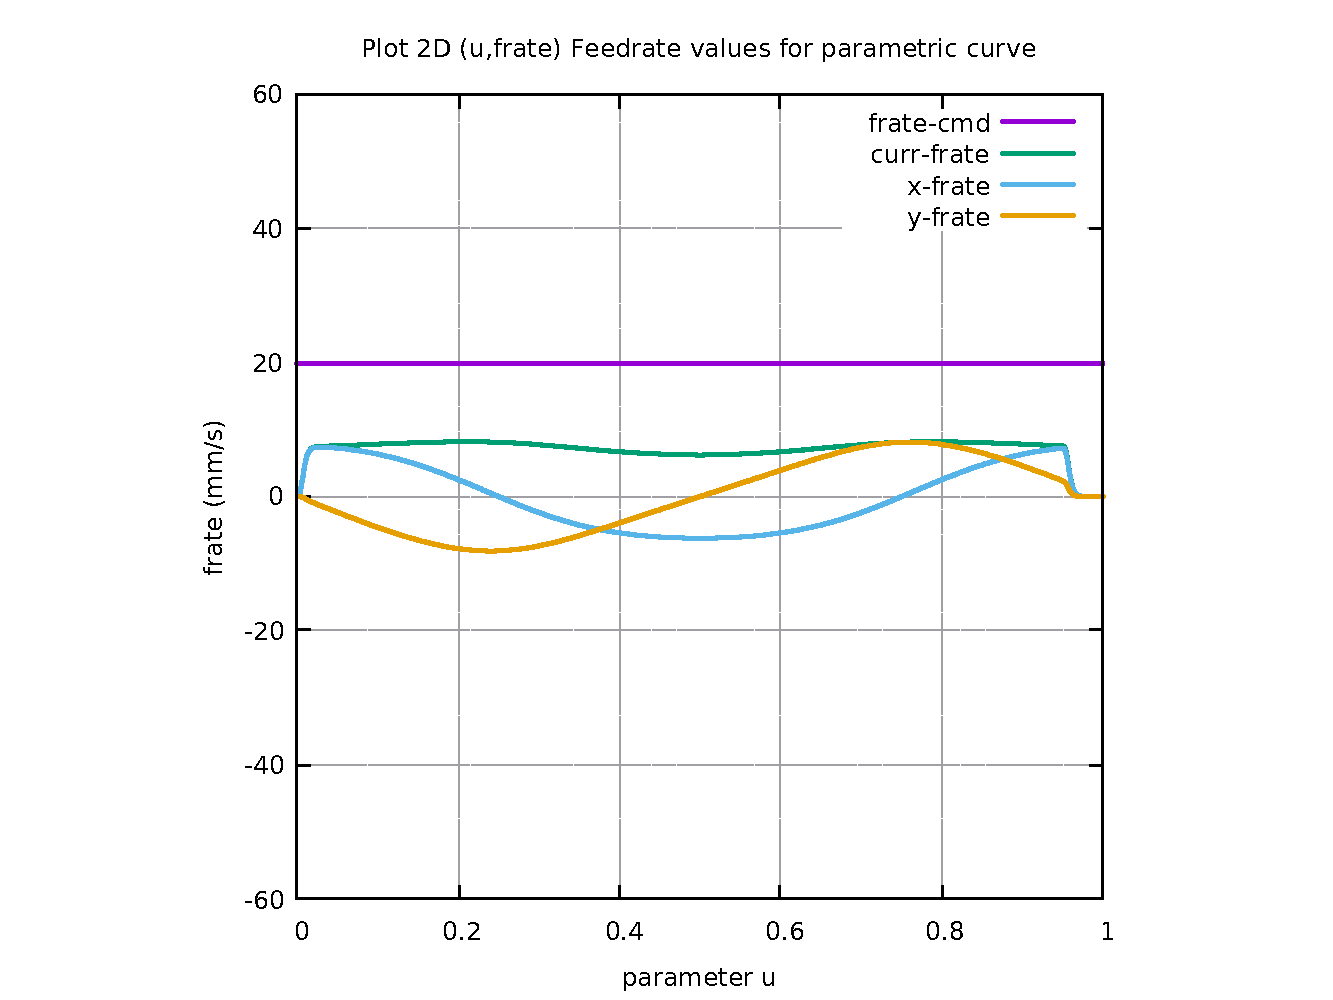
\includegraphics[width=1.00\textwidth]{Chap4/appendix/app-Circle/plots/28-img-Circle-FC20-FrateCmd-CurrFrate-X-Frate-Y-Frate.pdf}
\end{figure}


%% ==================================================
\clearpage
\pagebreak

\begin{figure}
	\caption     {Circle FC30 FrateCmd CurrFrate X-Frate Y-Frate}
	\label{29-img-Circle-FC30-FrateCmd-CurrFrate-X-Frate-Y-Frate.pdf}
	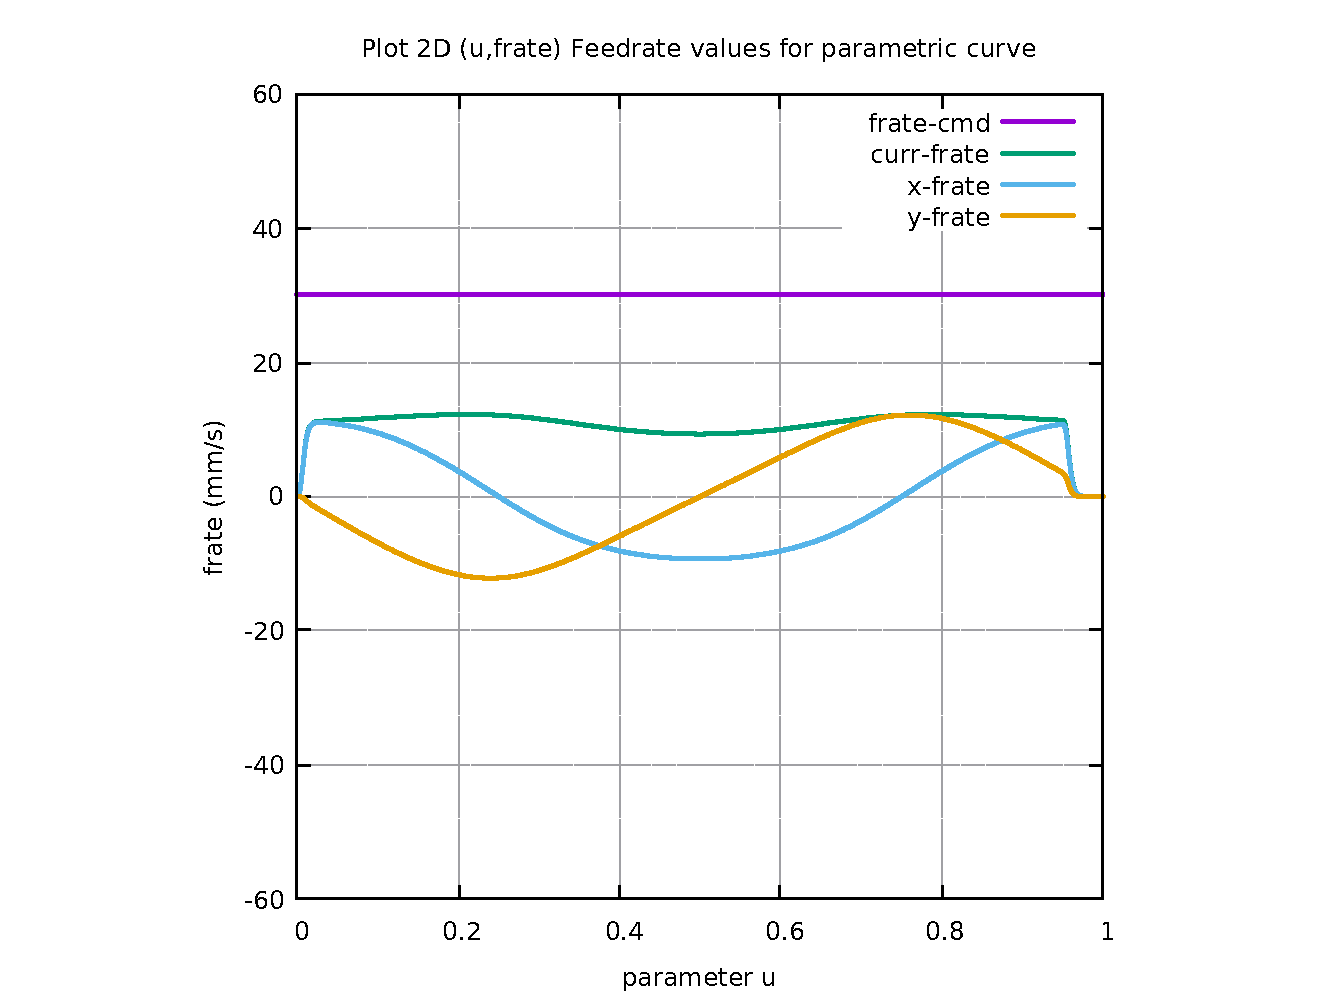
\includegraphics[width=1.00\textwidth]{Chap4/appendix/app-Circle/plots/29-img-Circle-FC30-FrateCmd-CurrFrate-X-Frate-Y-Frate.pdf}
\end{figure}


\begin{figure}
	\caption     {Circle FC40 FrateCmd CurrFrate X-Frate Y-Frate}
	\label{30-img-Circle-FC40-FrateCmd-CurrFrate-X-Frate-Y-Frate.pdf}
	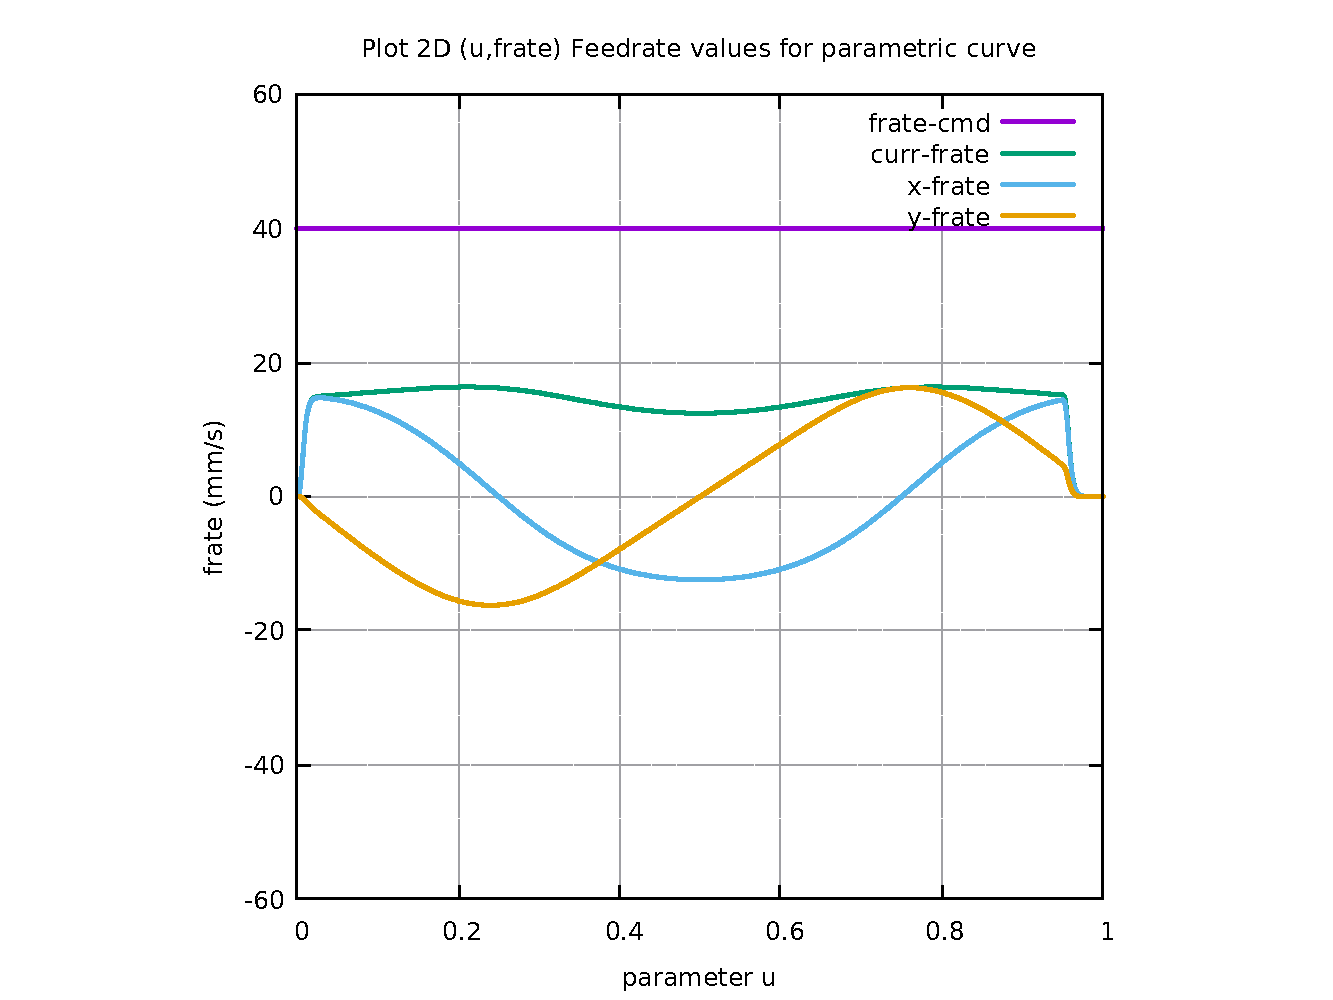
\includegraphics[width=1.00\textwidth]{Chap4/appendix/app-Circle/plots/30-img-Circle-FC40-FrateCmd-CurrFrate-X-Frate-Y-Frate.pdf}
\end{figure}


%% ==================================================
\clearpage
\pagebreak

\begin{figure}
	\caption     {Circle FC10 Four Components FeedrateLimit}
	\label{31-img-Circle-FC10-Four-Components-FeedrateLimit.pdf}
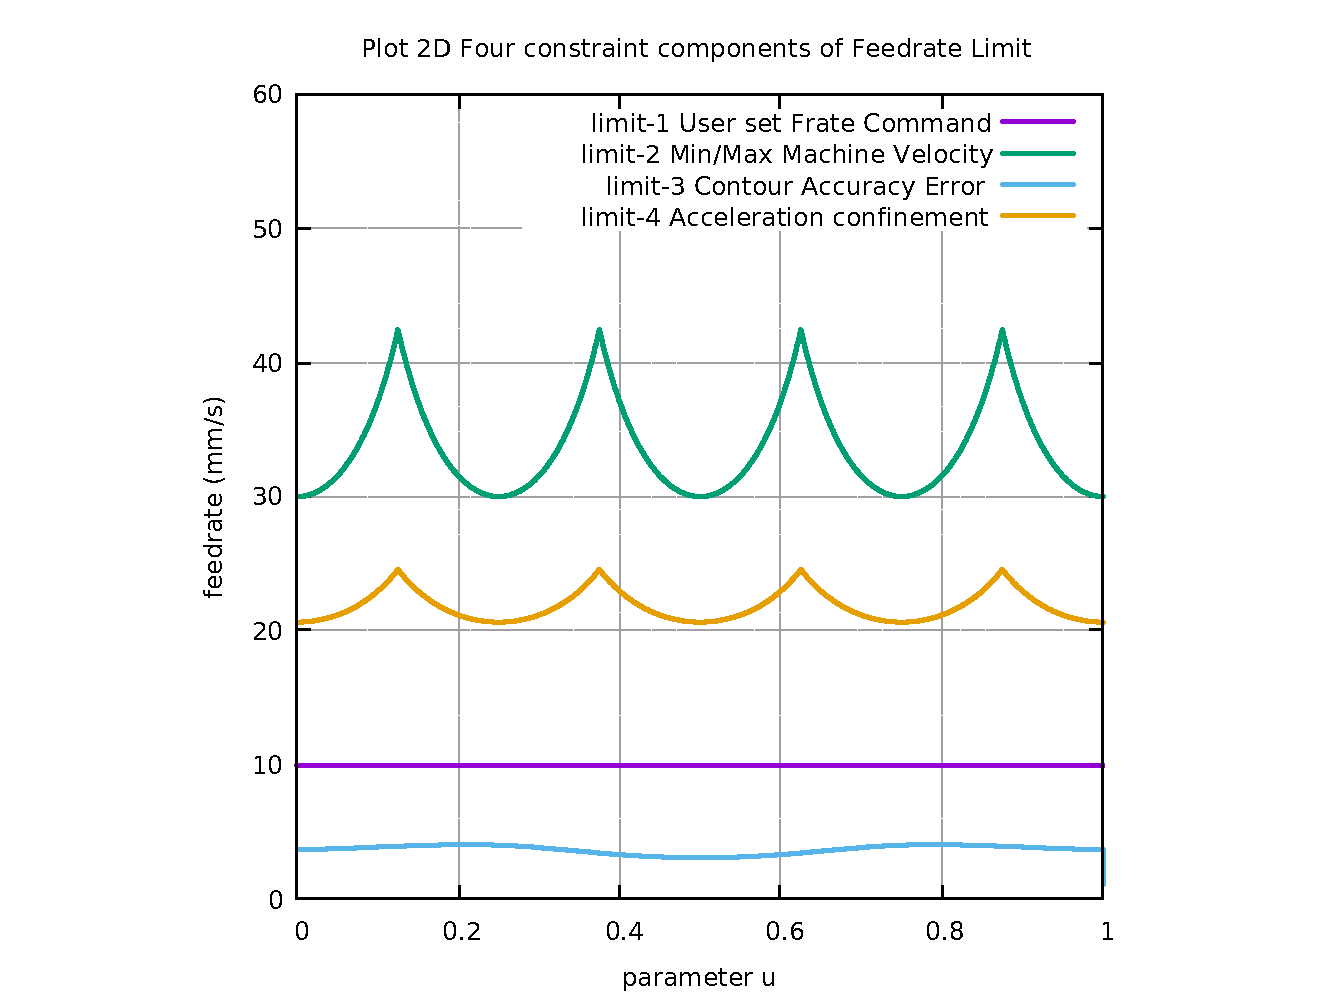
\includegraphics[width=1.00\textwidth]{Chap4/appendix/app-Circle/plots/31-img-Circle-FC10-Four-Components-FeedrateLimit.pdf}
\end{figure}


\begin{figure}
	\caption     {Circle FC20 Four Components FeedrateLimit}
	\label{32-img-Circle-FC20-Four-Components-FeedrateLimit.pdf}
	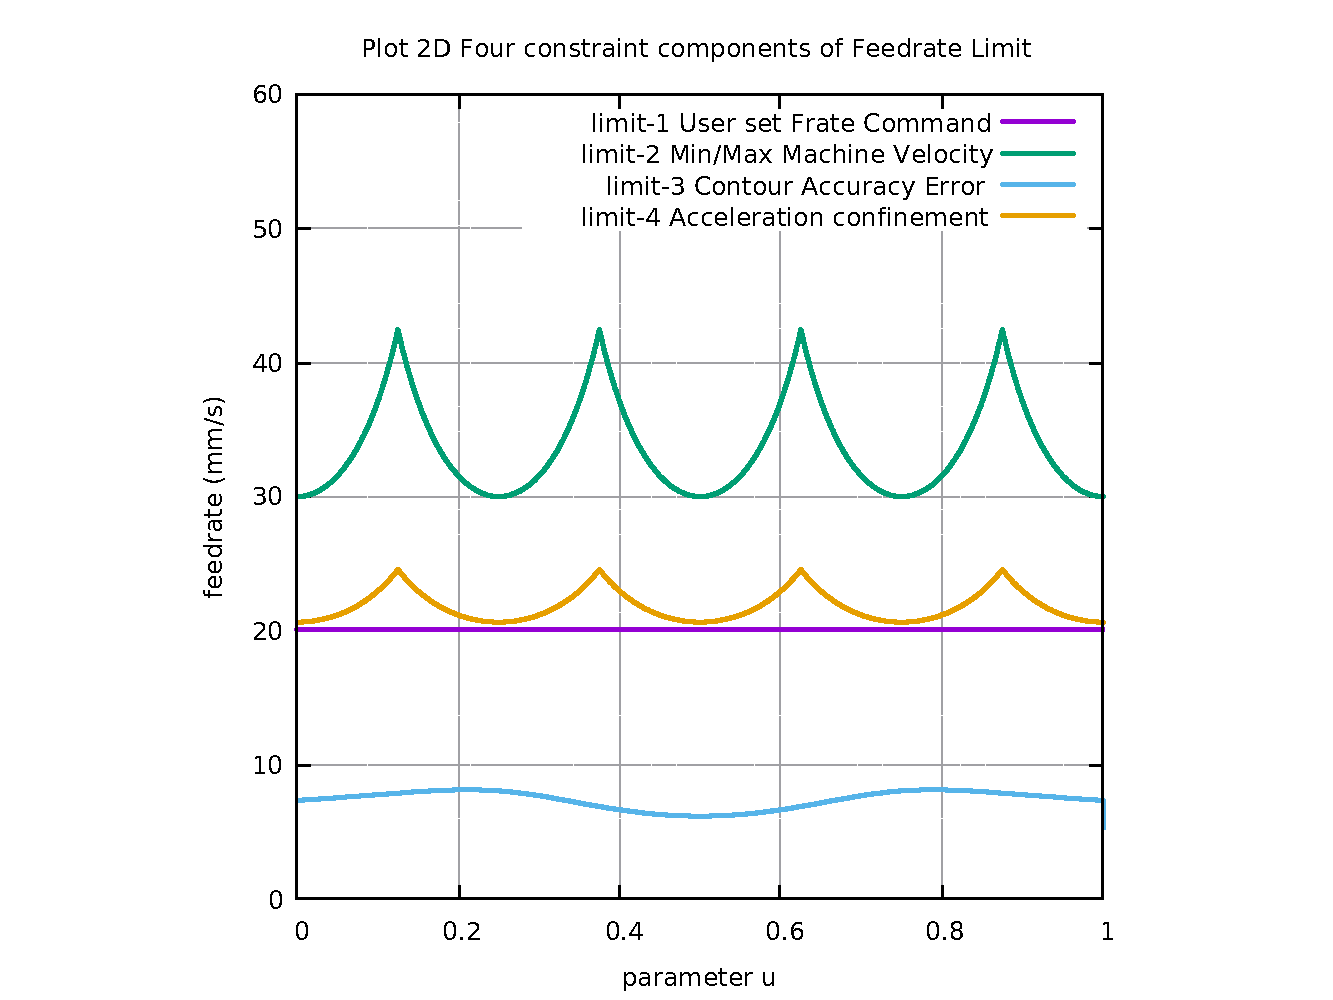
\includegraphics[width=1.00\textwidth]{Chap4/appendix/app-Circle/plots/32-img-Circle-FC20-Four-Components-FeedrateLimit.pdf}
\end{figure}


%% ==================================================
\clearpage
\pagebreak

\begin{figure}
	\caption     {Circle FC30 Four Components FeedrateLimit}
	\label{33-img-Circle-FC30-Four-Components-FeedrateLimit.pdf}
	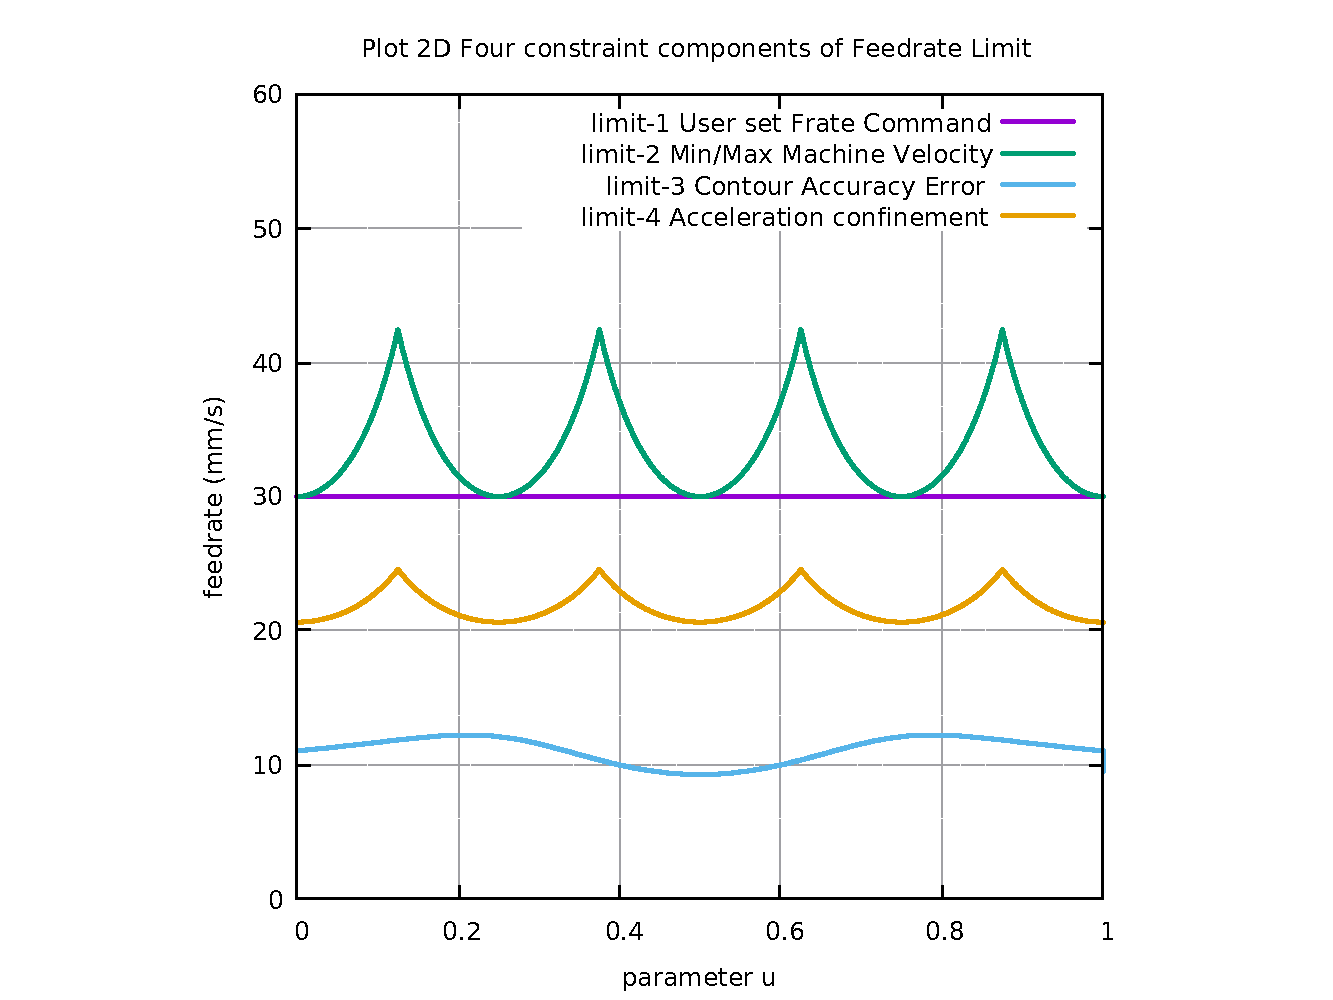
\includegraphics[width=1.00\textwidth]{Chap4/appendix/app-Circle/plots/33-img-Circle-FC30-Four-Components-FeedrateLimit.pdf}
\end{figure}


\begin{figure}
	\caption     {Circle FC40 Four Components FeedrateLimit}
	\label{34-img-Circle-FC40-Four-Components-FeedrateLimit.pdf}
	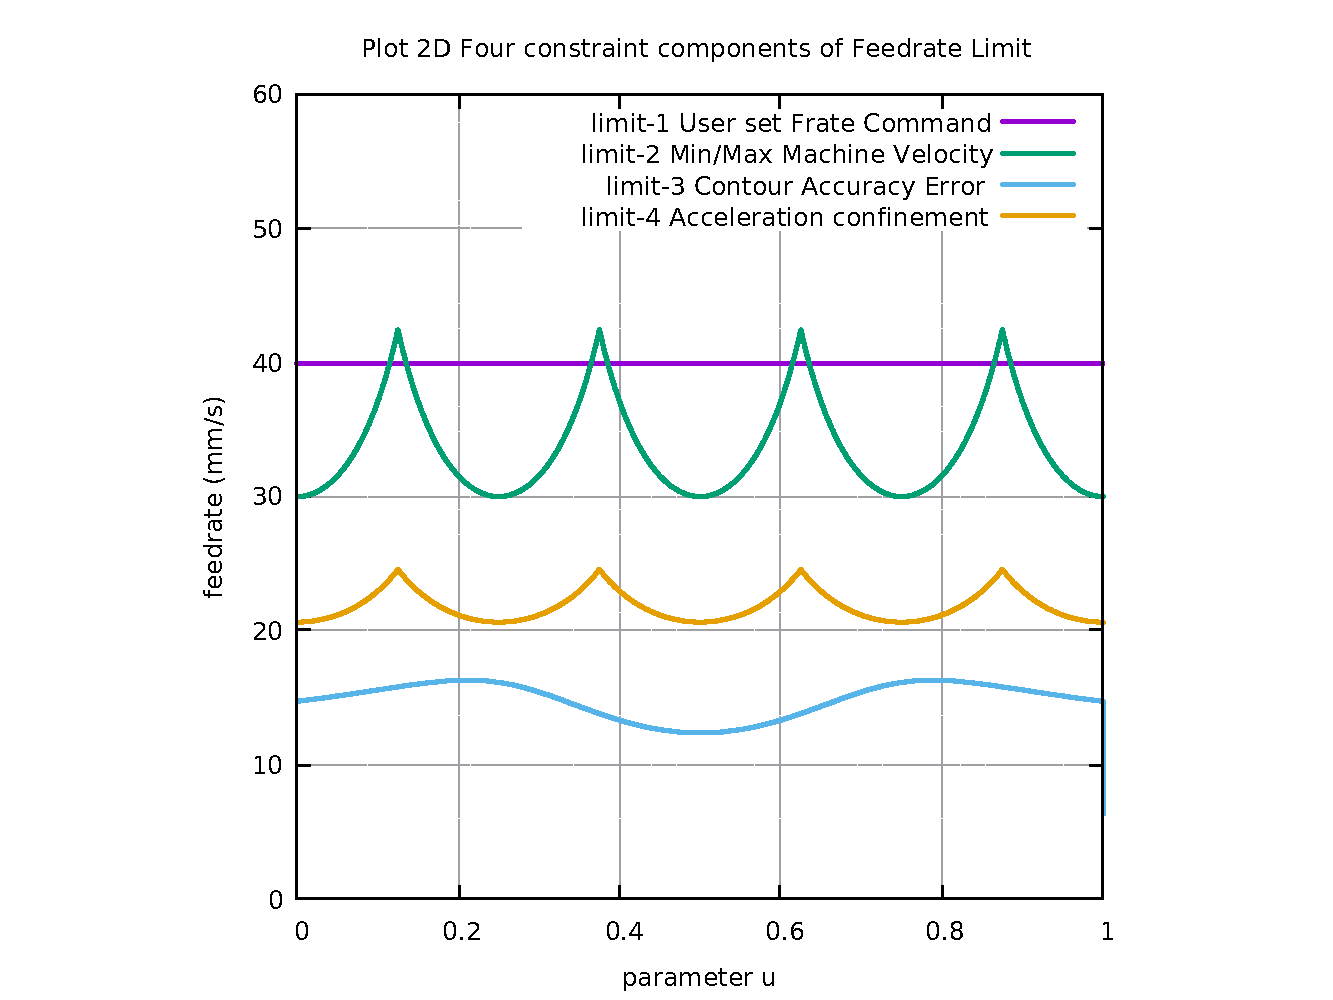
\includegraphics[width=1.00\textwidth]{Chap4/appendix/app-Circle/plots/34-img-Circle-FC40-Four-Components-FeedrateLimit.pdf}
\end{figure}

%% =======================================
\clearpage
\pagebreak

\begin{figure}
	\centering
	\caption     {Circle Histogram Points FC10 FC20 FC30 FC40}
	\label{35-img-Circle-Histogram-Points-FC10-FC20-FC30-FC40.pdf}
	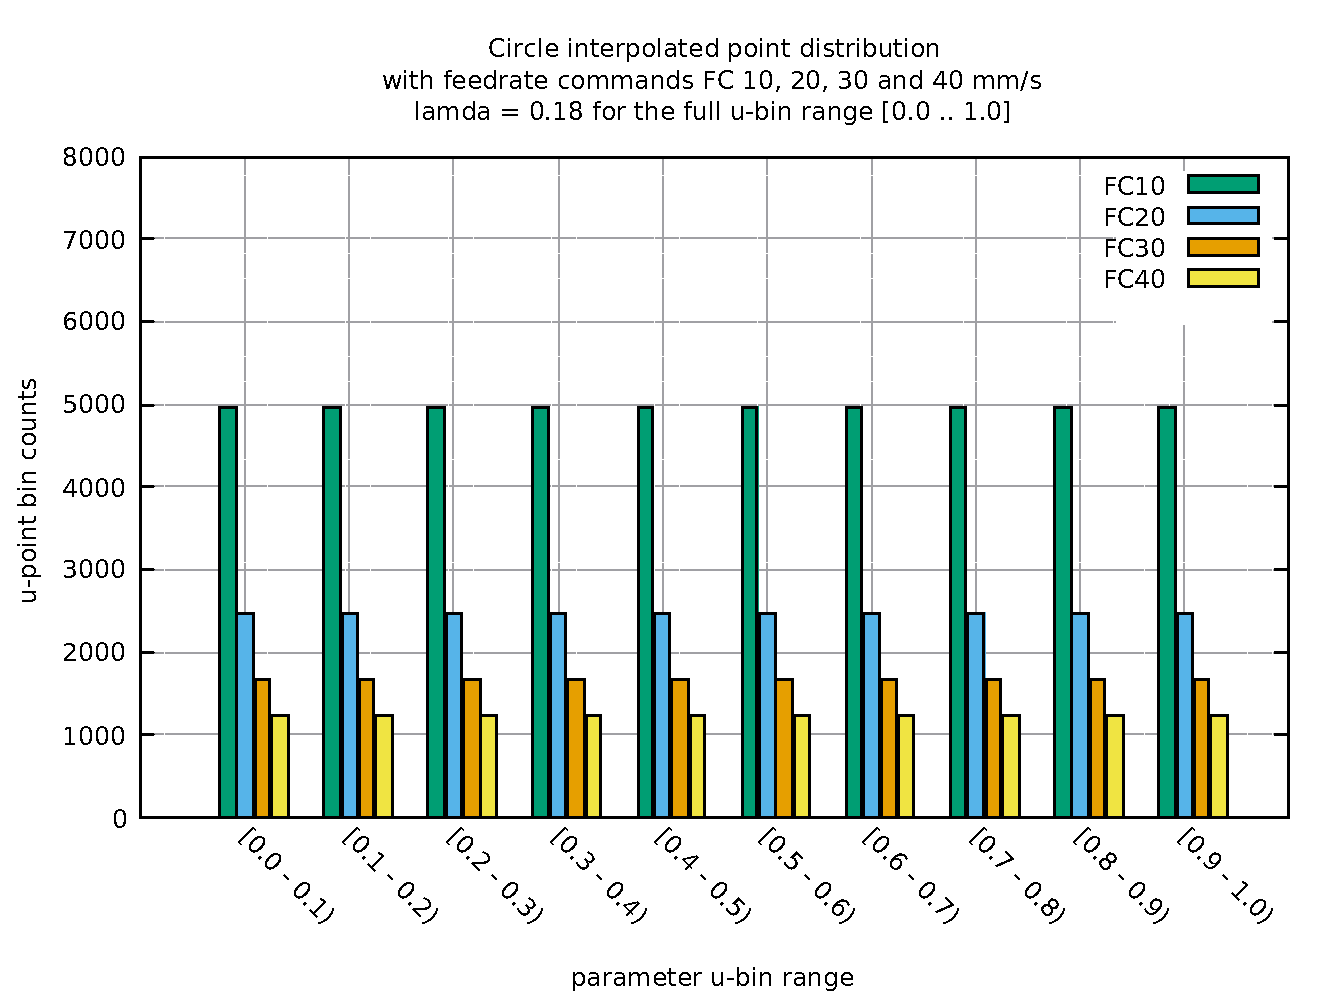
\includegraphics[width=1.00\textwidth]{Chap4/appendix/app-Circle/plots/35-img-Circle-Histogram-Points-FC10-FC20-FC30-FC40.pdf} 
\end{figure}


\begin{table}[ht]
%% \begin{center}
\caption    {Circle Table distribution of interpolated points}
\label  {tab-Circle Table distribution of interpolated points}
	
%% IMPORTANT TO SCALEBOX BELOW
\scalebox{0.80}{
		
%% START COPY AND PASTE BELOW HERE
%% FROM \begin{tabular} UNTIL \end{tabular)
%% Note: adjust last p{} to get line width correct
		
\begin{tabular}{ p{4.5cm} p{1.5cm} p{1.5cm} p{1.5cm} p{7.50cm} }
\hline
&		&		&		&		\\
BINS	&	FC10	&	FC20	&	FC30	&	FC40	\\
&		&		&		&		\\
0.0 - 0.1	&	4964	&	2482	&	1654	&	1241	\\
0.1 - 0.2	&	4964	&	2482	&	1655	&	1241	\\
0.2 - 0.3	&	4964	&	2482	&	1655	&	1241	\\
0.3 - 0.4	&	4964	&	2482	&	1655	&	1241	\\
0.4 - 0.5	&	4964	&	2482	&	1655	&	1242	\\
0.5 - 0.6	&	4964	&	2483	&	1655	&	1241	\\
0.6 - 0.7	&	4964	&	2482	&	1655	&	1241	\\
0.7 - 0.8	&	4964	&	2482	&	1655	&	1241	\\
0.8 - 0.9	&	4964	&	2482	&	1654	&	1242	\\
0.9 - 1.0	&	4965	&	2483	&	1656	&	1242	\\
&		&		&		&		\\
Tot Counts	&	49641	&	24822	&	16549	&	12413	\\
&		&		&		&		\\
\hline	
\end{tabular}
		
%% END COPY AND PASTE ABOVE HERE
		
}   %% IMPORTANT FOR SCALEBOX CLOSING
	
\hrule
\end{table}
%% \end{landscape}

%% CIRCLE SUMMARY TABLE
%% ========================================================
\clearpage
\pagebreak
\begin{landscape}
	
\begin{table}[ht]
%% \begin{center}
\caption       {Circle Table FC10-20-30-40 Run Performance data}
\label{tab-app4-Circle-Table-FC10-20-30-40-Run-Performance-data}

%% IMPORTANT TO SCALEBOX BELOW
\scalebox{0.90}{
			
%% START COPY AND PASTE BELOW HERE
%% FROM \begin{tabular} UNTIL \end{tabular)
			
\begin{tabular}{ p{0.2cm} p{8.80cm} p{4.00cm} p{4.0cm} p{4.00cm} p{4.0cm}}
\hline
				&		&		&		&		&		\\
				1	&	Curve Type	&	CIRCLE	&	CIRCLE	&	CIRCLE	&	CIRCLE	\\
				2	&	User Feedrate Command FC(mm/s)                   	&	FC10	&	FC20	&	FC30	&	FC40	\\
				3	&	User Lamda Acceleration Safety Factor	&	0.18	&	0.18	&	0.18	&	0.18	\\
				&		&		&		&		&		\\
				4	&	Total Iterpolated Points (TIP)	&	49641	&	24822	&	16549	&	12413	\\
				5	&	Total Sum-Chord-Error (SCE) (mm)	&	1.093913738449E-03	&	2.187639876000E-03	&	3.281178287065E-03	&	4.374701201686E-03	\\
				6	&	Ratio 1 = (SCE/TIP) = Chord-Error/Point	&	2.203694074232E-08	&	8.813665347893E-08	&	1.982824683989E-07	&	3.524573962041E-07	\\
				&		&		&		&		&		\\
				7	&	Total Sum-Arc-Length (SAL) (mm)	&	4.963785816452E+02	&	4.963771594934E+02	&	4.963757335444E+02	&	4.963942987341E+02	\\
				8	&	Total Sum-Chord-Length (SCL) (mm)	&	4.963785813150E+02	&	4.963771581682E+02	&	4.963757305630E+02	&	4.963942934342E+02	\\
				9	&	Difference = (SAL – SCL) (mm)	&	3.302195636934E-07	&	1.325165840171E-06	&	2.981455850204E-06	&	5.299917688717E-06	\\
				10	&	Percentage Difference = (SAL – SCL)/SAL	&	6.652574786747E-08	&	2.669675295946E-07	&	6.006449648363E-07	&	1.067683029848E-06	\\
				&		&		&		&		&		\\
				11	&	Ratio 2 = (SCE/SCL) = Chord Error/Chord-Length	&	2.203789163406E-06	&	4.407213023407E-06	&	6.610271383220E-06	&	8.812956271960E-06	\\
				&		&		&		&		&		\\
				12	&	Total Sum-Arc-Theta (SAT) (rad)	&	6.283146611127E+00	&	6.283002050952E+00	&	6.282857458743E+00	&	6.282965934945E+00	\\
				13	&	Total Sum-Arc-Area (SAA) (mm2)	&	5.235292684461E-05	&	2.093803820914E-04	&	4.710353817982E-04	&	8.373046676549E-04	\\
				&		&		&		&		&		\\
				14	&	Ratio 3 = (SAA/SCL) = Arc-Area/Chord-Length	&	2.203789163406E-06	&	4.407213023407E-06	&	6.610271383220E-06	&	8.812956271960E-06	\\
				&		&		&		&		&		\\
				15	&	Average-Chord-Error (ACE) (mm)	&	2.203694074232E-08	&	8.813665347893E-08	&	1.982824683989E-07	&	3.524573962041E-07	\\
				16	&	Average-Arc-Length (AAL) (mm)	&	9.999568526293E-03	&	1.999827402173E-02	&	2.999611636116E-02	&	3.999309528956E-02	\\
				17	&	Average-Chord-Length (ACL) (mm)	&	9.999568519641E-03	&	1.999827396834E-02	&	2.999611618099E-02	&	3.999309486257E-02	\\
				18	&	Average-Arc-Theta (AAT) (rad)	&	1.265742669445E-04	&	2.531325108155E-04	&	3.796747316136E-04	&	5.062009293381E-04	\\
				19	&	Average-Arc-Area (AAA) (mm2)	&	1.054652031519E-09	&	8.435614281914E-09	&	2.846479222856E-08	&	6.745928679140E-08	\\
				&		&		&		&		&		\\
				20	&	Algorithm actual runtime on computer (ART) (s) 	&	17.277667419	&	8.160163431	&	5.399371536	&	4.053925000	\\
				&		&		&		&		&	\\	
\hline				
\end{tabular}
			
%% END COPY AND PASTE		
}   %% IMPORTANT FOR SCALEBOX CLOSING
\end{table}
\end{landscape}

%% =====================================================
%% ==================================================
